%Version 3.1 December 2024
% See section 11 of the User Manual for version history
%
%%%%%%%%%%%%%%%%%%%%%%%%%%%%%%%%%%%%%%%%%%%%%%%%%%%%%%%%%%%%%%%%%%%%%%
%%                                                                 %%
%% Please do not use \input{...} to include other tex files.       %%
%% Submit your LaTeX manuscript as one .tex document.              %%
%%                                                                 %%
%% All additional figures and files should be attached             %%
%% separately and not embedded in the \TeX\ document itself.       %%
%%                                                                 %%
%%%%%%%%%%%%%%%%%%%%%%%%%%%%%%%%%%%%%%%%%%%%%%%%%%%%%%%%%%%%%%%%%%%%%

%%\documentclass[referee,sn-basic]{sn-jnl}% referee option is meant for double line spacing

%%=======================================================%%
%% to print line numbers in the margin use lineno option %%
%%=======================================================%%

%%\documentclass[lineno,pdflatex,sn-basic]{sn-jnl}% Basic Springer Nature Reference Style/Chemistry Reference Style

%%=========================================================================================%%
%% the documentclass is set to pdflatex as default. You can delete it if not appropriate.  %%
%%=========================================================================================%%

%%\documentclass[sn-basic]{sn-jnl}% Basic Springer Nature Reference Style/Chemistry Reference Style

%%Note: the following reference styles support Namedate and Numbered referencing. By default the style follows the most common style. To switch between the options you can add or remove �Numbered� in the optional parenthesis.
%%The option is available for: sn-basic.bst, sn-chicago.bst%

%%\documentclass[pdflatex,sn-nature]{sn-jnl}% Style for submissions to Nature Portfolio journals
%%\documentclass[pdflatex,sn-basic]{sn-jnl}% Basic Springer Nature Reference Style/Chemistry Reference Style
\documentclass[pdflatex,sn-mathphys-num]{sn-jnl}% Math and Physical Sciences Numbered Reference Style
%%\documentclass[pdflatex,sn-mathphys-ay]{sn-jnl}% Math and Physical Sciences Author Year Reference Style
%%\documentclass[pdflatex,sn-aps]{sn-jnl}% American Physical Society (APS) Reference Style
%%\documentclass[pdflatex,sn-vancouver-num]{sn-jnl}% Vancouver Numbered Reference Style
%%\documentclass[pdflatex,sn-vancouver-ay]{sn-jnl}% Vancouver Author Year Reference Style
%%\documentclass[pdflatex,sn-apa]{sn-jnl}% APA Reference Style
%%\documentclass[pdflatex,sn-chicago]{sn-jnl}% Chicago-based Humanities Reference Style

%%%% Standard Packages
\usepackage{algorithm}
\usepackage{algorithmicx}
\usepackage{algpseudocode}
\usepackage{amsmath,amssymb,amsfonts}
\usepackage{booktabs}
\usepackage{color}
\usepackage{listings}
\usepackage{lineno}

% Added by author
\usepackage{csquotes}
\usepackage{caption}
\usepackage{tabularx}
\usepackage{makecell}
\usepackage{cleveref}
\usepackage{setspace}
\usepackage{siunitx}
\usepackage{afterpage}
\usepackage{tikz}
\usetikzlibrary{positioning}
\usetikzlibrary{arrows}
\usetikzlibrary{calc}
\usetikzlibrary{shadows}
\usetikzlibrary{shapes.misc}
% \usepackage{showframe}
\usepackage[draft]{fixme}
\fxuselayouts{inline,nomargin}
\fxusetheme{color}
%%%%

%%%%%=============================================================================%%%%
%%%%  Remarks: This template is provided to aid authors with the preparation
%%%%  of original research articles intended for submission to journals published
%%%%  by Springer Nature. The guidance has been prepared in partnership with
%%%%  production teams to conform to Springer Nature technical requirements.
%%%%  Editorial and presentation requirements differ among journal portfolios and
%%%%  research disciplines. You may find sections in this template are irrelevant
%%%%  to your work and are empowered to omit any such section if allowed by the
%%%%  journal you intend to submit to. The submission guidelines and policies
%%%%  of the journal take precedence. A detailed User Manual is available in the
%%%%  template package for technical guidance.
%%%%%=============================================================================%%%%

%% as per the requirement new theorem styles can be included as shown below
% \theoremstyle{thmstyleone}%
% \newtheorem{theorem}{Theorem}%  meant for continuous numbers
% %%\newtheorem{theorem}{Theorem}[section]% meant for sectionwise numbers
% %% optional argument [theorem] produces theorem numbering sequence instead of independent numbers for Proposition
% \newtheorem{proposition}[theorem]{Proposition}%
% %%\newtheorem{proposition}{Proposition}% to get separate numbers for theorem and proposition etc.

% \theoremstyle{thmstyletwo}%
% \newtheorem{example}{Example}%
% \newtheorem{remark}{Remark}%

% \theoremstyle{thmstylethree}%
% \newtheorem{definition}{Definition}%

\raggedbottom
%%\unnumbered% uncomment this for unnumbered level heads


%% Recommended way to typeset C++
%% https://tex.stackexchange.com/questions/4302/prettiest-way-to-typeset-c-cplusplus
\def\CC{{C\nolinebreak[4]\hspace{-.05em}\raisebox{.4ex}{\tiny\bf ++}}}

% There are a lot of quotes in this document so make the command shorter.
\newcommand{\q}[1]{\enquote{#1}}

%% Acronyms
\usepackage[automake]{glossaries-extra}
\setabbreviationstyle[acronym]{long-short}
\makeglossaries

% Apparently the only way to prevent all the acronyms from generating spelling errors is to 
% disable ltex on the entire file.
% LTeX: enabled=false

\newabbreviation{ai}{AI}{Artificial Intelligence}
\newabbreviation{ar}{AR}{Augmented Reality}
\newabbreviation{asf}{ASF}{Amplitude Stereo Features}
\newabbreviation{cac}{CAC}{Cut And Clicks}
% \newabbreviation{cd}{CD}{Cochleagram Difference}
\newabbreviation{cd}{CD}{Compact Disc}
\newabbreviation{dft}{DFT}{Discrete Fourier Transform}
\newabbreviation{dirac}{DirAC}{Directional Audio Coding}
\newabbreviation{dl}{DL}{Deep Learning}
\newabbreviation[longplural=Directions of Arrival]{doa}{DOA}{Direction of Arrival}
\newabbreviation{dsp}{DSP}{Digital Signal Processing}
\newabbreviation{erb}{ERB}{Equivalent Rectangular Bandwidth}
\newabbreviation{fa}{FA}{Frequency-Azimuth}
\newabbreviation{faa}{FAA}{Frequency-Azimuth Analysis}
\newabbreviation{fft}{FFT}{Fast Fourier Transform}
\newabbreviation{fir}{FIR}{finite impulse response}
\newabbreviation{fmttm}{FMTTM}{Fly Me To The Moon}
\newabbreviation{genai}{Gen-AI}{Generative Artificial Intelligence}
\newabbreviation{iamf}{IAMF}{Immersive Audio Model and Formats}
\newabbreviation{daw}{DAW}{Digital Audio Workstation}
\newabbreviation{dj}{DJ}{Disc Jockey}

\newabbreviation{rq}{RQ}{research question}

\newabbreviation{iid}{IID}{Interaural Intensity Difference}
\newabbreviation{ipd}{IPD}{Interaural Phase Difference}
\newabbreviation{icpd}{ICPD}{Inter-channel Phase Difference}
\newabbreviation{ccpd}{CCPD}{Cross-channel Phase Difference}
\newabbreviation{ild}{ILD}{Interaural Level Difference}
\newabbreviation{ilr}{ILR}{Interaural Level Ratio}
\newabbreviation{cld}{CLD}{Channel Level Difference}
\newabbreviation{ccad}{CCAD}{Cross-channel Amplitude Difference}
\newabbreviation{icld}{ICLD}{Inter-channel Level Difference}
\newabbreviation{itd}{ITD}{Interaural Time Difference}
\newabbreviation{ictd}{ICTD}{Inter-channel Time Difference}
\newabbreviation{iacc}{IACC}{Interaural Cross Correlation}
\newabbreviation{iccc}{ICCC}{Inter-channel Cross Correlation}
\newabbreviation{icc}{ICC}{Inter-channel Correlation}
\newabbreviation{ic}{IC}{Inter-channel Coherence}
\newabbreviation{iac}{IAC}{Interaural Coherence}
\newabbreviation{itf}{ITF}{Inter-channel Transfer Function}
\newabbreviation{lev}{LEV}{Listener Envelopment}
\newabbreviation{dsd}{DSD}{Directional Loudness Distortion}
\newabbreviation{bms}{BMS}{Bivariate Mixture Space}
\newabbreviation{spl}{SPL}{Sound Pressure Level}
\newabbreviation{iir}{IIR}{Infinite Impulse Response}


\newabbreviation{ishst}{ISHST\textsuperscript{**}}{I Saw Her Standing There\textsuperscript{**}}
\newabbreviation{kks}{KKS}{The Knowledge Foundation}
\newabbreviation{lb}{LB}{Laser Beam}
\newabbreviation{lfe}{LFE}{Low Frequency Effects}
\newabbreviation{llm}{LLM}{Large Language Model}
\newabbreviation{lufs}{LUFS}{Loudness Units Full Scale}
\newabbreviation{mirex}{MIREX}{Music Information Retrieval Evaluation eXchange}
\newabbreviation{mir}{MIR}{Music Information Retrieval}
\newabbreviation{ml}{ML}{Machine Learning}
\newabbreviation{mtg}{MTG}{Music Technology Group}
\newabbreviation{m}{M}{Manifesto}
\newabbreviation{pc}{PC}{Panning Coefficients}
\newabbreviation{ph}{PH}{Panning Histogram}
\newabbreviation{pi}{PI}{Panning Index}
\newabbreviation{picoc}{PICOC}{Population, Intervention, Comparison, Outcome, Context}
\newabbreviation{psf}{PSF}{Phase Stereo Features}
\newabbreviation{qm}{QM}{Qualitative Model}
\newabbreviation{rms}{RMS}{Root Mean Squared}
\newabbreviation{rm}{RM\textsuperscript{*}}{'Round Midnight\textsuperscript{*}} 
\newabbreviation{simpl}{SIMPL}{stereo-input mixed-to-panned level}
\newabbreviation{sip}{SIP}{Stereo Image Profile}
\newabbreviation{slr}{SLR}{Systematic Literature Review}
\newabbreviation{spf}{SPF}{Stereo Panning Features}
\newabbreviation{sps}{SPS}{Stereo Panning Spectrum}
\newabbreviation{ssps}{SSPS}{Spectral Stereo Phase Spread}
\newabbreviation{stft}{STFT}{Short-time Fourier Transform}
\newabbreviation{tf}{TF}{time-frequency}
\newabbreviation{titt}{TITT}{This Is The Thing}
\newabbreviation{vr}{VR}{Virtual Reality}
\newabbreviation{peaq}{PEAQ}{Objective Measurements of Perceived Audio Quality}
\newabbreviation{peaqmc}{PEAQ-MC}{Objective Measurements of Perceived Audio Quality - Multi Channel}
\newabbreviation{cnn}{CNN}{Convolutional Neural Network}

\newabbreviation{ica}{ICA}{Independent Component Analysis}
\newabbreviation{pca}{PCA}{Principal Component Analysis}
\newabbreviation{pqmf}{PQMF}{Pseudo Quadrature Mirror Filter}
\newabbreviation{mpeg}{MPEG}{Moving Picture Experts Group}
\newabbreviation{3gpp}{3GPP}{3rd Generation Partnership Project}

\newabbreviation{asw}{ASW}{Apparent Source Width}
\newabbreviation{fwhm}{FWHM}{Full Width Half Maximum}
\newabbreviation{lef}{LEF}{Lateral Energy Fraction}
\newabbreviation{iqr}{IQR}{Interquartile Range}
\newabbreviation{amt}{AMT}{Auditory Modelling Toolbox}
\newabbreviation{qestral}{QESTRAL}{Quality Evaluation of Spatial Transmission and Reproduction using an Artificial Listener}
\newabbreviation{bcc}{BCC}{Binaural Cue Coding}
\newabbreviation{ps}{PS}{Parametric Stereo}
\newabbreviation{saoc}{SAOC}{Spatial Audio Object Coding}
\newabbreviation{gccphat}{GCC-PHAT}{Generalized Cross Correlation with Phase Transform}
\newabbreviation{mp3}{MP3}{MPEG layer 3}
\newabbreviation{aac}{AAC}{Advanced Audio Coding}
\newabbreviation{ivas}{IVAS}{Immersive Voice and Audio Services}
\newabbreviation{sofa}{SOFA}{Spatially Oriented Format for Acoustics}

\newabbreviation{ir}{IR}{Impulse Response}
\newabbreviation{hrir}{HRIR}{Head-Related Impulse Response}
\newabbreviation{hrtf}{HRTF}{Head-Related Transfer Function}
\newabbreviation{midi}{MIDI}{Musical Instrument Digital Interface}
\newabbreviation{vi}{VI}{Virtual Instrument}
\newabbreviation{mushra}{MUSHRA}{MUlti Stimulus Hidden Reference and Anchor}
\newabbreviation{bsseval}{BSS\_EVAL}{Blind Source Separation Evaluation}
\newabbreviation{psd}{PSS}{Perceptual Spectral Difference}
\newabbreviation{bamq}{BAM-Q}{Binaural-Auditory-Model-based Quality}
\newabbreviation{tff}{TFF}{Time-Frequency Filter}
\newabbreviation{pco}{PCO}{Population, Context, Outcome}
\newabbreviation{wos}{WOS}{Web Of Science}
\newabbreviation{ss}{SS}{Semantic Scholar}
\newabbreviation{cpu}{CPU}{Central Processing Unit}
\newabbreviation{flop}{FLOP}{Floating Point Operation}

\newabbreviation{csv}{CSV}{Comma Separated Variable}
\newabbreviation{tsv}{TSV}{Tab Separated Variable}
\newabbreviation{api}{API}{Application Programming Interface}
\newabbreviation{doi}{DOI}{Digital Object Identifier}
\newabbreviation{url}{URL}{Universal Resource Locator}
\newabbreviation{prisma}{PRISMA}{Preferred Reporting Items for Systematic reviews and Meta-Analyses}
\newabbreviation{adress}{ADRess}{Azimuth Discrimination and Resynthesis}
\newabbreviation{agr}{AGR}{Automatic Genre Recognition}
\newabbreviation{som}{SOM}{Self Organising Map}
\newabbreviation{iresap}{IRESAP}{Information Retrieval in Embedded Systems for Audiovisual Artistic Processes}
\newabbreviation{mdu}{MDU}{Mälardalen Universitet}
\newabbreviation{kmh}{KMH}{Kungliga Musikhögskolan}




% datasets
\newabbreviation{boma}{BOMA}{{Bang \& Olufsen Music for Archimedes}}
\newabbreviation{uiowamis}{UIowaMIS}{University of Iowa Musical Instrument Samples}
% \newabbreviation{}{}{Bach10}
\newabbreviation{btpab}{BTPAB}{ByTeDance paired ambisonic and binaural}
\newabbreviation{dsd100}{DSD100}{Demixing Secret Database}
\newabbreviation{asascbrm}{ASASCBRM}{Database for Automatic Spatial Audio Scene Classification in Binaural Recordings of Music}
\newabbreviation{daoc}{DAOC}{Denon anechoic orchestral collection}
% \newabbreviation{}{}{FAIR-Play}
\newabbreviation{fma}{FMA}{Free Music Archive}
% \newabbreviation{}{}{MedleyDB}
% \newabbreviation{}{}{MedleyDB 2.0}
% \newabbreviation{}{}{MUSDB18}
% \newabbreviation{}{}{MUSDB18-HQ}
\newabbreviation{quasi}{QUASI}{QUaero Audio SIgnals}
\newabbreviation{rwc}{RWC}{Real World Computing}
\newabbreviation{sqam}{SQAM}{EBU Sound Quality Assessment Material}
% \newabbreviation{}{}{Slakh}
\newabbreviation{urmp}{URMP}{University of Rochester Multi-Modal Music Performance}
% \newabbreviation{}{}{ccMixter}
\newabbreviation{arsso}{ARSSO}{Anechoic Recording System for Symphony Orchestra}
\newabbreviation{rioossr}{RIOOSSR}{Recordings of Italian opera orchestra and soloists in a silent room}
\newabbreviation{msss}{MSSS}{Mixing Secrets for The Small Studio}
\newabbreviation{tss}{TSS}{Telefunken Studio Sessions}
\newabbreviation{mtgj}{MTGJ}{Music Technology Group Jamendo}
% \newabbreviation{}{}{Audio and Acoustic Signal Processing Technical Committee Online Resources}
\newabbreviation{maestro}{MAESTRO}{MIDI and Audio Edited for Synchronous TRacks and Organization}
% \newabbreviation{}{}{FiloSax}
% \newabbreviation{}{}{Gamelan Music Dataset}
% \newabbreviation{}{}{mobygratis}


% Journals
\newabbreviation{jaes}{JAES}{Journal of the Audio Engineering Society}
\newabbreviation{eurasip}{EURASIP}{European Association for Signal Processing}

%% Numbers of papers in specific categories.
\newcommand{\nTotal}{4313}
\newcommand{\nFollowedReferences}{15}
\newcommand{\nRecommendationService}{5}
\newcommand{\nPeers}{5}
\newcommand{\nPreprints}{9}
\newcommand{\nDuplicateByDOI}{960}
\newcommand{\nDuplicateByTitleAndYear}{456}
\newcommand{\nRemovedBeforeScreening}{1416}
\newcommand{\nScreened}{2897}
\newcommand{\nExcludedAfterScreening}{2226}
\newcommand{\nSoughtForRetrieval}{671}
\newcommand{\nNotRetrieved}{45}
\newcommand{\nAssessedForEligibility}{626}
\newcommand{\nExcludedAfterAssessment}{460}
\newcommand{\nExcludedNotVeryRelevant}{139}
\newcommand{\nIncluded}{166}
\newcommand{\nIncludedVeryRelevant}{27}
\newcommand{\nAssessedMaybe}{84}
\newcommand{\nAssessedDefinitely}{542}
\newcommand{\nIncludedMaybe}{3}
\newcommand{\nIncludedDefinitely}{163}

%% Listing style for database queries
\lstdefinestyle{databasequery}{
  basicstyle=\ttfamily\footnotesize,
  breakatwhitespace=true,
  breaklines=true,
  captionpos=t,
  keepspaces=true,
  numbers=none,
  showspaces=false,
  showstringspaces=false,
  showtabs=false,
  frame=tbrl,
  breakindent=0pt,
  columns=fullflexible,
}
\lstset{style=databasequery}

%% Listing style for python
\definecolor{deepblue}{rgb}{0,0,0.5}
\definecolor{deepgreen}{rgb}{0,0.5,0}
\lstdefinestyle{python}{
    language=Python,
    basicstyle=\ttfamily\footnotesize,
    frame=tb,
    showstringspaces=false,
    keywordstyle=\color{deepblue},
    stringstyle=\color{deepgreen},
}

\begin{document}

\doublespacing
\linenumbers

\title[Article Title]{A Systematic Literature Review of Methods to Describe the Stereo Image of Recorded Music}

%%=============================================================%%
%% GivenName	-> \fnm{Joergen W.}
%% Particle	-> \spfx{van der} -> surname prefix
%% FamilyName	-> \sur{Ploeg}
%% Suffix	-> \sfx{IV}
%% \author*[1,2]{\fnm{Joergen W.} \spfx{van der} \sur{Ploeg}
%%  \sfx{IV}}\email{iauthor@gmail.com}
%%=============================================================%%

\author[*]{\fnm{Richard} \sur{Mitic}}\email{richard.mitic@mdu.se}

% \author[2,3]{\fnm{Second} \sur{Author}}\email{iiauthor@gmail.com}
% \equalcont{These authors contributed equally to this work.}

% \author[1,2]{\fnm{Third} \sur{Author}}\email{iiiauthor@gmail.com}
% \equalcont{These authors contributed equally to this work.}

\affil*[]{\orgdiv{School of Innovation, Design and Engineering}, \orgname{M{\"a}lardalens Universitetet}, \orgaddress{\street{Universitetsplan 1}, \city{V{\"a}ster{\r a}s}, \postcode{72220}, \state{V{\"a}stmanlands l{\"a}n}, \country{Sweden}}}

% \affil[2]{\orgdiv{Department}, \orgname{Organization}, \orgaddress{\street{Street}, \city{City}, \postcode{10587}, \state{State}, \country{Country}}}

% \affil[3]{\orgdiv{Department}, \orgname{Organization}, \orgaddress{\street{Street}, \city{City}, \postcode{610101}, \state{State}, \country{Country}}}

%%==================================%%
%% Sample for unstructured abstract %%
%%==================================%%

\abstract{

Recorded music contains a wealth of spatial information which is of interest for many types of audio research. Describing a recording's spatial features has been attempted in the past, but was limited in scope. Since then, the amount of recorded music available for research has exploded, and it is therefore pertinent to find descriptors of spatial features that can be used to analyse new datasets. To that end, a \gls{slr} was conducted in order to ascertain all existing methods to describe the spatial features of stereophonic musical audio. The Scopus, \gls{wos}, and \gls{ss} databases were searched on 30\textsuperscript{th} September 2024, and articles were deemed eligible if the method they described included any extraction of spatial information from a music audio signal. The spatial features in question were recorded, along with any downstream tasks they were applied to and audio datasets they were applied on. Links and similarities were drawn between studies to identify the core methods of describing stereo field. \nIncluded~articles were included, with \nIncludedVeryRelevant~of those deemed \q{very relevant}. The fundamental methods of extracting spatial information are detailed and a framework for creating a custom \gls{sip} is drawn up, followed by suggestions for future research. The review was limited by the substantial volume of literature to be assessed by a single reviewer, although this wide breadth served to mitigate bias by gathering at least one example of all existing \gls{sip} methods. The inconsistent application of terminology within the existing literature presented a significant challenge. The work was funded in part by \gls{kks}.
}

%%================================%%
%% Sample for structured abstract %%
%%================================%%

% \abstract{\textbf{Purpose:} The abstract serves both as a general introduction to the topic and as a brief, non-technical summary of the main results and their implications. The abstract must not include subheadings (unless expressly permitted in the journal's Instructions to Authors), equations or citations. As a guide the abstract should not exceed 200 words. Most journals do not set a hard limit however authors are advised to check the author instructions for the journal they are submitting to.
%
% \textbf{Methods:} The abstract serves both as a general introduction to the topic and as a brief, non-technical summary of the main results and their implications. The abstract must not include subheadings (unless expressly permitted in the journal's Instructions to Authors), equations or citations. As a guide the abstract should not exceed 200 words. Most journals do not set a hard limit however authors are advised to check the author instructions for the journal they are submitting to.
%
% \textbf{Results:} The abstract serves both as a general introduction to the topic and as a brief, non-technical summary of the main results and their implications. The abstract must not include subheadings (unless expressly permitted in the journal's Instructions to Authors), equations or citations. As a guide the abstract should not exceed 200 words. Most journals do not set a hard limit however authors are advised to check the author instructions for the journal they are submitting to.
%
% \textbf{Conclusion:} The abstract serves both as a general introduction to the topic and as a brief, non-technical summary of the main results and their implications. The abstract must not include subheadings (unless expressly permitted in the journal's Instructions to Authors), equations or citations. As a guide the abstract should not exceed 200 words. Most journals do not set a hard limit however authors are advised to check the author instructions for the journal they are submitting to.}

\keywords{Music Information Retrieval, Stereo Image, Systematic Literature Review}

%%\pacs[JEL Classification]{D8, H51}

%%\pacs[MSC Classification]{35A01, 65L10, 65L12, 65L20, 65L70}

\maketitle

\listoffixmes

\section{Introduction}
\label{sec:intro}
The extraction of spatial information from musical audio signals has long been a goal for digital music practitioners, with downstream uses such as classification, recommendation, format conversion, and even musicology. However, until the recent development of object-based audio, it was not common practice to include any such information in music metadata, and it must therefore be derived after-the-fact from the final musical mix. With the new availability of very large musical datasets there exists an opportunity to gain insights into musicians' use of spaciousness in their work.

It is imperative to recognize that the gamut of spatial processing in audio research is enormous, and the terminology, keywords, and article structure somewhat non-standardized. Many studies include the extraction of spatial information in their methods, and while said information may be enough to describe stereo field, the articles are written from the perspective of the downstream task rather than the spatial features themselves. Consequently, \textit{very relevant} literature is difficult to find using simple searches, yet increasing the search radius results in excessive amounts of \textit{semi-relevant} literature. This represents a missed opportunity for \q{cross-pollination} between adjacent (but usually independent) audio research fields, and to that end, this \gls{slr} aims to determine all currently available methods to describe the stereo field of recorded music. It follows the \gls{prisma} guidelines \cite{pagePRISMA2020Statement2021}.

\subsection{Previous reviews}
\label{sec:previous_reviews}
Reviews of techniques to extract spatial information from audio are generally rare, with the few examples being tailored to a specific use cases. For example, \cite{cobosOverviewMachineLearning2022} gives an overview of \gls{ml}-based techniques for the capture, processing, and rendering of spatial audio. The targeted use cases are gaming, \gls{ar}/\gls{vr}, teleconferencing, and entertainment applications. While binaural audio is mentioned as a spatial format, other stereophonic recordings are not, nor is the focus on musical audio. The authors also state that their review is \q{representative ... [but not] exhaustive}. In a similar vein, \cite{yangAudioAugmentedReality2022} is an \gls{slr} of the technologies and applications of spatial audio in \gls{ar}. The authors state that it is the first systematic review in the field, but the audio sections are focused on synthesis rather than analysis, and (like the former) musical audio is not targeted. A more recent review \cite{zhuASAudioSurveyAdvanced2025} focused specifically on spatial audio, mentioning music as a use case. It too only references binaural audio (and not stereophonic more generally) as a spatial format, and is focused on research performed from 2022 onwards. It does, however, give an excellent overview of input and output audio representations, spatial audio tasks, available datasets, and evaluation metrics.

\subsection{New aims and scope of this review}
\label{sec:new_aims}
To fill gaps in previous reviews, this \gls{slr} focuses specifically on techniques to describe the spatial features of stereophonic musical audio, extracting them from previous literature and gathering them in a single place for reference by the audio research community. The aforementioned lack of standardization will be normalized such that future researchers can share a common footing and language. See \cref{sec:syntheses} for a detailed explanation of specific outcomes.

% Specifically, the research question being addressed is
% \\\\
% \noindent\textit{What methods exist to describe the spatial features of stereophonic music recordings?}
% \\\\

A list of sonic qualities that represent audio \q{spaciousness} is defined in \cite{bergSystematicEvaluationPerceived2003}, from which it is possible to infer that any audio signal with more than one channel is eligible to contain spatial information. One may argue that some spatial attributes (namely \q{depth}, \q{distance}, and \q{reverberation}) can also be extracted from monophonic signals \cite{sarroffMeasurementsSpaciousnessStereophonic2008}. Nonetheless, monophonic audio is deemed out of scope for this review. Conversely, while many studies act on audio with more than two channels, they are still deemed relevant if the underlying techniques could be applied to stereophonic audio.


\section{Methods}\label{sec:methods}

This section defines all processes for performing the review, and discusses some known limitations.

\subsection{Search process}\label{sec:search_process}

The review follows the \gls{pco} protocol \cite{pollockHowSystematicReview2018}. The population is defined as \q{music}, the context as \q{stereo}, and the outcome as \q{spatial information}. Since these terms and their synonyms are often not standardized, a list of negative search terms were also included to exclude some obvious false positives. Several very specific terms that were already known to the author were also included, and any article using those terms was included in the initial search result. The full lists of synonyms, specific terms, and negative terms used to form search queries, plus the search queries themselves can be found in appendix \ref{ap:search_terms}. The search was performed on 30\textsuperscript{th} September 2024.


\begin{table}[htbp]
    \centering
    \caption{Databases used for article search}
    \begin{tabularx}{\textwidth}{llX}
        \toprule
          & Database & Description \\
        \midrule
        1 & Scopus \cite{Scopus} & The largest database of scientific articles, indexing a majority of computer-science publishers. \\
        2 & \glsxtrlong{wos} \cite{WebScience} & Another well-respected general scientific database that acts to fill gaps in Scopus. \\
        3 & \glsxtrlong{ss} \cite{SemanticScholar} & A general-purpose scientific database created via web-scraping that tends to surface more \q{grey} publications such as theses, commercial white papers, and pre-prints, but can be prone to errors and false records. \\
        \bottomrule
    \end{tabularx}
    \label{tab:databases}
\end{table}

\Cref{tab:databases} shows the databases that were searched, and their precedence. Both Scopus and \gls{wos} have a browser-based search functionality accepting advanced queries, from which the results can be exported as \gls{csv}/\gls{tsv} files. \gls{ss} provides an \gls{api} endpoint that can be used to perform similar advanced searches \cite{SemanticScholarAcademic}. It was found during initial searches that although the \gls{ss} \gls{api} accepts negative terms, it often wrongly excluded relevant articles. Negative terms were therefore omitted from the \gls{ss} query. The data exported from the searches was \gls{url}, title, abstract, authors, publication year, publication source, \gls{doi}, and citation count of each study. A full dataset of the collected search results for all databases is included with this manuscript as an additional file.

\subsection{Initial screening}
\label{sec:initial_screening}
The initial list of articles was filtered to remove duplicates, firstly identifying them by \gls{doi}, and then by title and publication year when \gls{doi} was not available. Since there are can be differences in formatting between the databases, the titles were first \q{normalized} by converting to lower case and removing all non-alphanumeric characters. Articles were marked as duplicates if the normalized title and publication year exactly matched one previously seen in the list. See appendix \ref{app:filter_code} for pseudocode that describes the automatic filtering process.

A first pass was then performed to make obvious exclusions. The title and abstract of each paper was read, and the article was rejected if any of the following were not true:

\begin{itemize}
    \item Database record was valid.
    \item Title and abstract were written in English.
    \item Document was available for reading.
    \item Document described some research\footnote{Other document types were e.g. book review, conference proceedings, patents, etc.}.
    % \item Document was not the proceedings of a conference.
    % \item Document was not a patent.
    \item Subject of the study was audio.
    \item Described method included the extraction of spatial features from an audio signal at any point.
\end{itemize}

Some duplicates were also identified manually and rejected at this stage. Note that the conditions of the audio comprising at least two channels and being musical was not assessed during the screening as it was very often not obvious from the title and abstract. If the reviewer was unsure about whether an article should be rejected or not, it was marked as \q{unclear} and revisited at a later stage.

\subsection{Review process}
\label{sec:full_assessment}
After the initial pass, all non-rejected articles and all articles marked as \q{unclear} with a publication year of 2020 or later were obtained and read in full. They were assessed (and possibly rejected) based on the same criteria mentioned in \cref{sec:initial_screening}, plus two additional conditions:

\begin{itemize}
    \item The audio signal comprised at least two channels
    \item The audio signal was musical
    % \item The downstream task related to a description of the spatial features
\end{itemize}

To assess whether an audio signal is musical or not, it must meet the condition that it contains a recording of at least one musical instrument (including singing voice), or that the study specifically stated with it was applicable to music. Studies using both musical and non-musical signals were also included.

While it is common to exclude reports based on the impact factor or citation count \cite{carrera-riveraHowtoConductSystematic2022}, an initial scan of the search results revealed that some very obviously relevant studies had very few, or even zero citations (e.g. \cite{yangUpmixingStyleTransfer2022}) or were published as pre-prints only (e.g. \cite{ziemerGoniometersArePowerful2023}). Therefore, citation count and publication venue were not taken into account.

Since the number of relevant studies from the initial assessment was high, a further selection process labelled those deemed \q{very relevant} to the aim described in \cref{sec:new_aims}. This process filtered studies based on their \q{downstream task} (see \cref{tab:data_extraction}), selecting tasks that are relevant to the extraction or interpretation or spatial information in large audio corpora.

\subsection{Data extraction}
\label{sec:data_extraction}
For each study included in the review, the following data was collected:

\newcolumntype{f}{X}
\newcolumntype{s}{>{\hsize=.44\hsize}X}

\begin{table}[htbp]
  \renewcommand{\arraystretch}{1.3} % This table is hard to read without a bit of white space between lines
  \centering
  \caption{Data extracted from reviewed articles}
  \begin{tabularx}{\textwidth}{sff}
      \toprule
      Data & Description & Examples \\
      \midrule
      Audio model & The channel count or standard paradigm that the audio signal follows & stereo, binaural, ambisonic, mic array \\
      Contents of signal & A high-level description of what the audio contained & music, speech, noise \\
      Specific audio configurations & More detail about the signal contents or how it was recorded/created & reverberant, synthetic binaural, orchestral \\
      Datasets & Any audio datasets that were used in the creation of the audio signal & \gls{fma}, \gls{mtgj}, MedleyDB \\
      Downstream tasks & The specific tasks that the spatial information was used (or was intended to be used) for & Source separation, \glsxtrshort{mir}, classification, compression \\
      Novel mechanism category & A high-level category of the articles main contribution & \glsxtrshort{dsp}, \glsxtrshort{ml}, psychoacoustic test \\
      Spatial attributes & The specific spatial information that was extracted from the audio signal & \glsxtrshort{doa}, panning histogram, cochleagram \\
      Novelty & A record of whether the article describes a new spatial feature or referenced one from the literature & novel, referenced, modified \\
      Evaluation technique & The technique by which the scientific claims were verified & Objective metrics, subjective test, simulations \\
      \bottomrule
  \end{tabularx}
  \label{tab:data_extraction}
\end{table}

Note that the options in each category are not mutually exclusive, e.g. \cite{fallerParametricCodingSpatial2004} describes \gls{bcc} which, while originally intended for the compression of multichannel signals, is also used for stereo. An additional example is \cite{tzanetakisStereoPanningInformation2010} which states that it's downstream task is \gls{mir}, and then provides proof of the method's effectiveness on a classification task.


\subsection{Syntheses}
\label{sec:syntheses}

The primary synthesis is an exhaustive list of methods to generate a \gls{sip} for musical audio, plus a thorough analysis of  their underlying extraction techniques, what musical features they are able to detect. Complementary to that is an explanation and normalization of their terminology, drawing links where studies are using similar techniques and differentiating between homonymous terms.

Following that, a framework of how to choose or form a spatial descriptor that is suitable for any particular task. The data extraction process differentiates between traditional \gls{dsp} and newer \gls{ml}/\gls{dl} spatial features, and it will be noted which tasks are currently benefiting from modern techniques, thereby giving inspiration for how to incorporate them in other tasks.

In addition, a list of useful audio datasets and experiment validation techniques will be formed so that any future researchers can find tools suitable for their tasks. Propositions for future research will also be given based on what is missing from the search results.

\subsection{Limitations}
Several limitations were uncovered during the review process. Firstly, due to the wide research questions and non-standardized formats of audio-related article abstracts, the number of article requiring review was very high. Only a single reviewer was tasked with reading all articles. This introduces a potential source of bias. However, the review's wide breadth was also a point of strength since the aim was to gather at least one example of all existing \gls{sip} algorithms. It is difficult to assess the impact of audio processing-related articles since they typically do not receive many citations and the publication venue and other related information is often missing from the databases. The solution was to assess each article equally, which created more manual work.

In addition, the non-standardized terminology meant that the database search queries (see appendix \ref{app:database_queries}) contain many synonyms for \q{spatial information}. The list was built iteratively over several initial searches, but there is still a chance that some missing keywords would have been beneficial to include. However, since this review is not concerned with the absolute number of search results for each term, this limitation is largely mitigated as long as at least one example of any given spatial descriptor was present in the results. Similarly, while the search process included specific terms for commercial spatial audio formats, information about them (and their underlying algorithms) is typically not public and hence was absent from the search results.

There is likely a bias regarding the publication venue of the articles sought for retrieval since some specific journals were not available through library subscriptions. Articles appearing potentially relevant were sought out via other methods (internet searches or direct contact with the authors) as a mitigation. Several doctoral theses were surfaced in the search results, and while they were relevant they were difficult to categorize in the review's framework since they typically contain multiple studies and hence fall into multiple categories. The accuracy of the data extracted from them could therefore be unreliable.

The assessment of \gls{dl}-related papers presented a few challenges. Firstly it is quite common to simply cite the audio dataset used, rather than describing the format and contents of the audio. Additionally, due to the black-box nature of \gls{dl}, the trained network often \textit{does} learn spatial features, but it is debatable whether that constitutes a spatial description (see \cref{sec:borderline} for examples).


\section{Results}
\label{sec:results}

The search initially identified \nTotal~studies, of which \nRemovedBeforeScreening~were removed before screening. \nExcludedAfterScreening~were excluded the after reading the title and abstract, leaving \nSoughtForRetrieval~that were sought for retrieval. Out of those, \nNotRetrieved~could not be retrieved and \nExcludedAfterAssessment~were rejected, leaving \nIncluded~that were included in the review. \nIncludedVeryRelevant~of those were deemed \q{very relevant} due to their downstream task. Using those \nIncluded~studies as a seed, \nFollowedReferences~studies were added by following references, \nRecommendationService~studies were found using the \gls{ss} recommendation service, and \nPeers~studies were recommended by peers. A full flow diagram of study inclusion and rejection is shown in figure \ref{fig:rejection_flow}.

\begin{figure}[htb]
\caption{\gls{prisma} flow diagram.}
\label{fig:rejection_flow}
\bigskip
\centering
\resizebox{0.95\linewidth}{!}{
  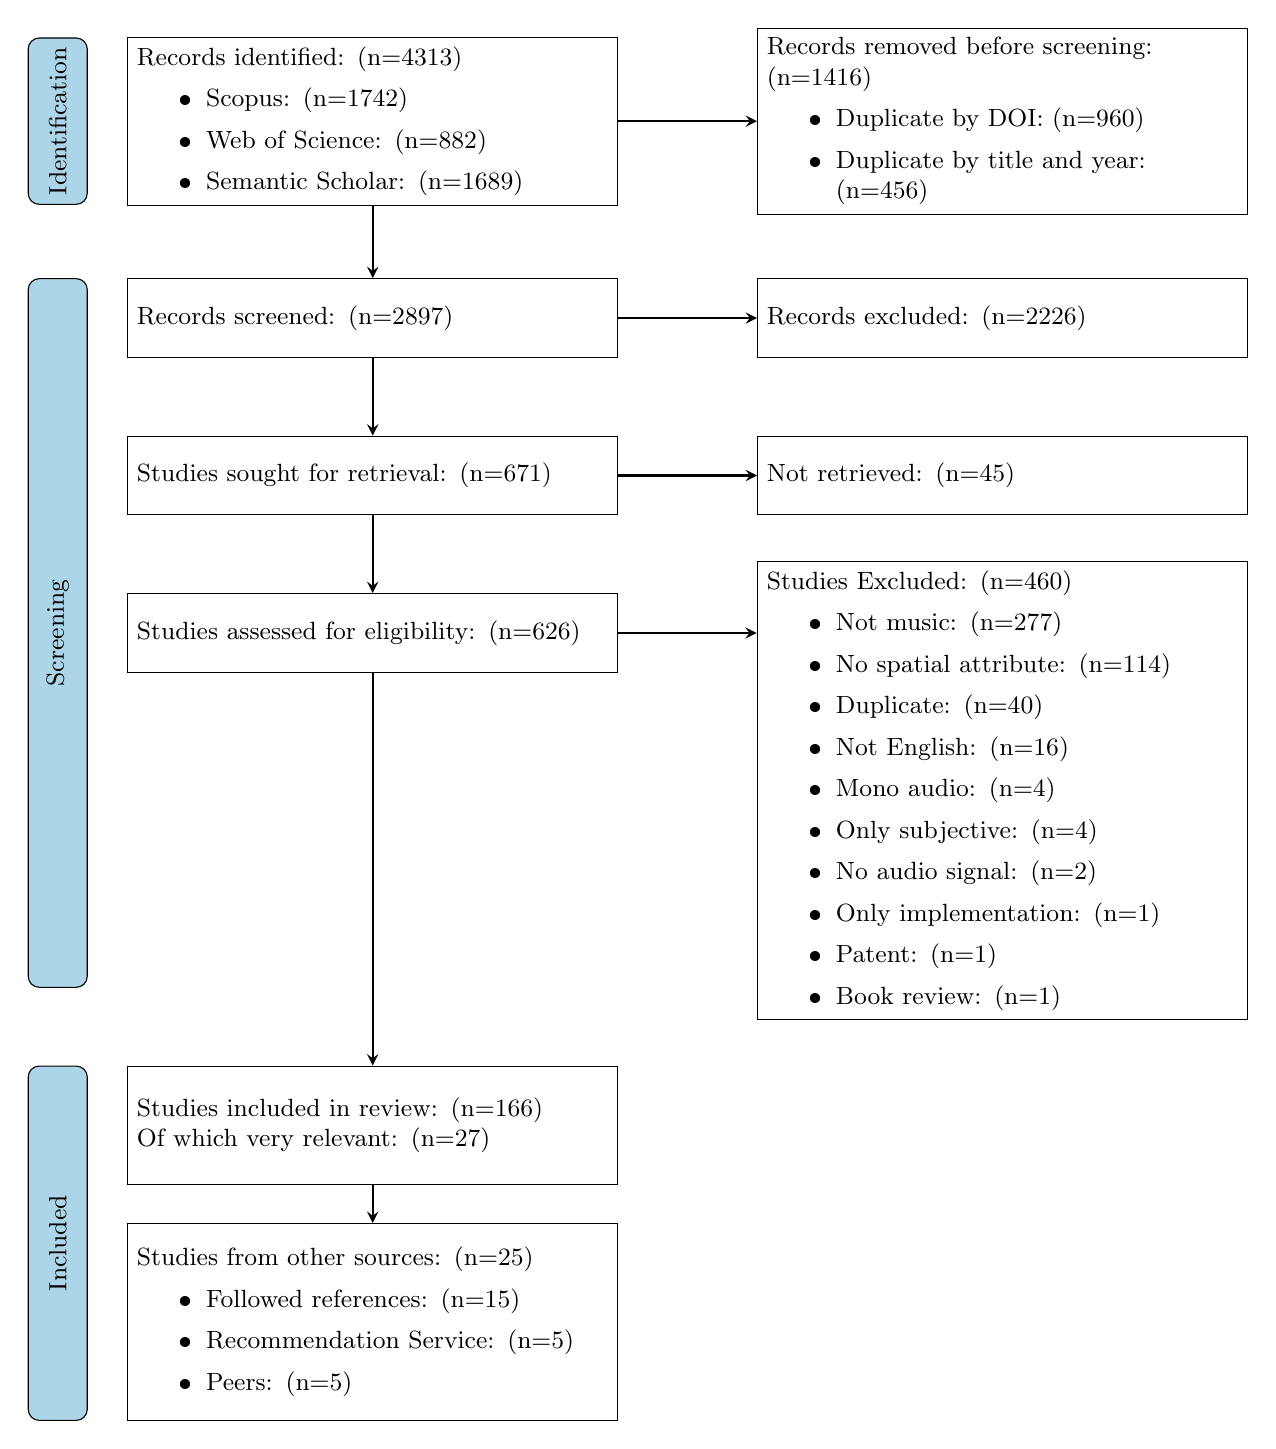
\begin{tikzpicture}[>=latex, font={\small}, node distance=2cm]
\tikzstyle{textrect} = [rectangle, minimum width=6cm, text width=5.99cm, minimum height=1cm, draw=black]
\tikzstyle{bluerect} = [rectangle, rounded corners, minimum width=1.5cm, minimum height=0.75cm, text centered, draw=black, fill=cyan!60!gray!45!white, rotate=90]
\tikzstyle{arrow} = [thick,->,>=stealth]
\node (identification_section) [bluerect, minimum width=2cm, yshift=4cm] {Identification};
\node (databases) [textrect, minimum height=2cm] {Records identified: (n=4313) \begin{itemize}\small\item Scopus: (n=1742)\item Web of Science: (n=882)\item Semantic Scholar: (n=1689)\end{itemize} };
\node (removed_before_screening) [textrect, right of=databases, xshift=6cm, minimum height=2cm] {Records removed before screening: (n=1416) \begin{itemize}\small\item Duplicate by DOI: (n=960)\item Duplicate by title and year: (n=456)\end{itemize} };
\node (screening_section) [bluerect, minimum width=9cm, yshift=4cm, xshift=-6.5cm] {Screening};
\node (screened) [textrect, below of=databases, yshift=-0.5cm] {Records screened: (n=2897)};
\node (excluded) [textrect, right of=screened, xshift=6cm] {Records excluded: (n=2226)};
\node (sought) [textrect, below of=screened] {Studies sought for retrieval: (n=671)};
\node (not_retrieved) [textrect, right of=sought, xshift=6cm] {Not retrieved: (n=45)};
\node (assessed) [textrect, below of=sought] {Studies assessed for eligibility: (n=626)};
\node (arrowanchor) [right of=assessed, xshift=3cm] {};
\node (rep_excluded) [textrect, right of=assessed, xshift=6cm, yshift=-2cm, minimum height=5cm] {Studies Excluded: (n=460) \begin{itemize}\small\item Not music: (n=277)\item No spatial attribute: (n=114)\item Duplicate: (n=40)\item Not English: (n=16)\item Mono audio: (n=4)\item Only subjective: (n=4)\item No audio signal: (n=2)\item Only implementation: (n=1)\item Patent: (n=1)\item Book review: (n=1)\end{itemize}};
\node (included) [textrect, below of=assessed, yshift=-4.25cm, minimum height=1.5cm] {Studies included in review: (n=166)\\Of which very relevant: (n=27)};
\node (included_section) [bluerect, left of=included, minimum width=4.5cm, yshift=4cm, xshift=0.5cm] {Included};
\node (othersources) [textrect, below of=included, yshift=-0.5cm, minimum height=2.5cm] {Studies from other sources: (n=25) \begin{itemize}\small\item Followed references: (n=15)\item Recommendation Service: (n=5)\item Peers: (n=5)\end{itemize} };
\draw [arrow] (databases) -- (removed_before_screening);
\draw [arrow] (databases) -- (screened);
\draw [arrow] (screened) -- (excluded);
\draw [arrow] (screened) -- (sought);
\draw [arrow] (sought) -- (not_retrieved);
\draw [arrow] (sought) -- (assessed);
\draw [arrow] (assessed.east) -- (arrowanchor);
\draw [arrow] (assessed) -- (included);
\draw [arrow] (included) -- (othersources);
\end{tikzpicture}

}
\end{figure}

As mentioned in \cref{sec:full_assessment}, some studies were marked as \q{unclear} during the initial screening. As a metric for the judgement of the reviewer, the number of studies assessed and eventually included are shown in \cref{tab:inclusion_ratios}. It shows that a far lower proportion of \q{unclear} studies were eventually included, implying that the reviewer's judgement was largely correct.

\begin{table}[h]
  \caption{Proportions of studies that were included in the review, split by clarity.}
  \label{tab:inclusion_ratios}
  \begin{tabular}{rccc}
\toprule
 & Assessed & Included & Proportion \\
\midrule
Obvious & 542 & 163 & 30\% \\
Unclear & 84 & 3 & 4\% \\
Total & 626 & 166 & 27\% \\
\bottomrule
\end{tabular}

\end{table}


\subsection{Borderline studies}
\label{sec:borderline}

Some studies presented edge cases during assessment. The following non-exhaustive list gives some examples of such studies, explaining why they were either included or excluded.

\begin{itemize}
    \item Inclusions
    \begin{itemize}
        \item \cite{pollowMeasuringDirectivitiesNatural2009} describes a method that acts on audio from a large microphone array rather than recorded music, but it is included because it mentions the nuances of using phase and intensity differences to estimate sound directivity.
        \item \cite{bourbonInvestigationImmersiveContemporary2023} uses multichannel renderings of object-based audio as the source, but was included because the method acts on pairs of channels as opposed to all channels simultaneously.
        \item \cite{fernandezEnhancingBinauralRendering2022} is primarily focused on the rendering of binaural microphone array signals, but was included because it references several useful algorithms for calculating spatial attributes of audio.
    \end{itemize}
    \item{Exclusions}
    \begin{itemize}
        \item \cite{lindauSpatialAudioQuality2014} contains a useful list of spatial audio terms, but doesn't describe any audio processing.
        \item \cite{coloneReverseEngineeringNonlinear2023} describes a method for predicting panning positions of stems in a stereo mix, but required access to those stems in order to function.
        \item \cite{felipeAcousticSceneClassification2017} uses stereo features to aid in the classification of binaural scenes, but does so by extracting monophonic features from each channel.
        \item \cite{sierraMultimodalMethodologyMusic2023} is focused on capturing spatial audio for \gls{mir} purposes, but simply outlines the capture process and choice of spatial format rather than deriving any spatial information.
        \item \cite{pulkkiFirstOrderDirectionalAudio2017} is a software implementation of the underlying spatial processing technique, which is described academically elsewhere in the literature.
    \end{itemize}
\end{itemize}




\subsection{Very Relevant Studies}
\label{sec:very_relevant_studies}

The \nIncludedVeryRelevant~studies deemed to be very relevant are those whose downstream task was at least one of \q{\gls{mir}}, \q{analysis}, \q{spatial analysis}, \q{musicology}, \q{psychoacoustics}, \q{visualization}, or \q{classification}. A full list of downstream tasks can be found in appendix \ref{app:downstream_tasks}. These studies tend to fall into tightly-related cohorts, often referencing each other. This section will summarize each study and draw links between them.

The earliest is \cite{supperOnsetGuidedSpatialAnalyser2005} -- a doctoral thesis defining methods for spatial analysis of binaural signals for use in the broadcasting industry. \cite{dewhirstModellingPerceivedSpatial2008} (another doctoral thesis) expands on \cite{supperOnsetGuidedSpatialAnalyser2005}, combining it with a binaural hearing model and an \gls{iacc} -based stereo width estimator \cite{masonImplementationApplicationBinaural2006} to create an artificial listener with the intention of assessing perceived sound at arbitrary (i.e. non-sweet-spot) listening positions.

A method to estimate amplitude panning position in the time-frequency domain (named \gls{pi}) was defined in \cite{avendanoFrequencyDomainTechniques2002,avendanoFrequencydomainSourceIdentification2003} and demonstrated for upmix and source separation tasks. \cite{tzanetakisStereoPanningFeatures2007} and its  extension \cite{tzanetakisStereoPanningInformation2010} define the \gls{spf} -- a descriptor of amplitude panning based on the \gls{pi} (although renamed to \gls{sps}). In turn, \cite{colonelReverseEngineeringRecording2021} uses \gls{spf} as a measure of similarity between two mixes of the same musical stems, and \cite{dalemanarangoArchivingSonicEphemeral2021} used the \gls{sps} to visualize artistic audio recordings and \gls{spf} as a measure of similarity between those recordings.

\cite{sarroffMeasurementsSpaciousnessStereophonic2008} defines a spatial descriptor named \gls{ph}, which is based on the \gls{fa} plane defined in \cite{barrySoundSourceSeparation2004}. The \gls{ph} is also collapsed into a single measure of \q{stereo width}, which the same author uses in \cite{sarroffPredictingPerceivedSpaciousness2009,sarroffComputationalModelPerceived2011} to create a computational model of perceived spaciousness. Notably, these studies also use monophonic descriptors, including a prediction of the extent of reverberation in the recording.

The concept of a \gls{ph} is used by several other studies, although under different names and with different mathematical definitions. \cite{takanenBinauralAuditoryModel2012} generates likelihood histograms of the \gls{doa} of sound sources from measurements of the \gls{ild} and \gls{itd} in binaural correlograms, from which a measurement of stereo width is also derived. A major difference from the previously mentioned works is that the method requires calibration using a recording of background noise, and reference \gls{ild}/\gls{itd} values from which the \gls{doa} is calculated. \cite{gomezMusicSimilaritySystems2008} defines another \gls{ph} which is based on the \gls{pi} from \cite{avendanoFrequencyDomainTechniques2002}. Furthermore, it defines a method of \gls{ph} quantization with the intention of allowing simple similarity measurement of music recordings in a lower-dimensional, non-perceptual domain. Differing slightly from other studies, \cite{prestiVisualizationManipulationStereophonic2014} focuses mostly on the visualization of stereo audio. It transforms \gls{tf} domain \gls{iid} and \gls{ipd} into two cues - \q{position} and \q{clarity} - which are then used to create several visualizations including a \gls{ph}. The same author expanded on this idea in \cite{prestiBivariateMixtureSpace2023}, defining a transformation from time-domain stereophonic signal into a generic \gls{bms}, which in turn is used for visualization and panning estimation (among others).

\cite{tardieuProductionEffectAudio2011} provides two alternative descriptors of panning features - \gls{asf} for amplitude panning and \gls{psf} for phase panning. They are created from time-domain cochleagrams and frequency-domain spectrograms respectively, and are demonstrated on a decade classification task.

\cite{harmaClassificationTimefrequencyRegions2011,harmaStereoAudioClassification2011} collectively demonstrate a new paradigm of \gls{sip} classification. As a precursor, a novel signal model is introduced that defines seven classes of stereo field. Subsequently, it is shown audio clips falling into six of the seven classes can be identified, first using a feed-forward neural network and then purely analytically. The inputs to the classifiers are cross correlations between the two channels and their variances (in \gls{tf} domain). The downstream tasks are the aforementioned classification itself, as well as audio enhancement, audio manipulation, and upmixing.

\cite{youSpatialLocalizationEvaluation2012} presents a method of comparing a degraded signal with its original in the spatial domain. It uses differences in \gls{iid} and \gls{itd} within audio sub-bands, the primary use case being objective assessment of spatial compression algorithms. With a similar use case of predicting the perceptual quality of binaural renderings of microphone arrays, \cite{nowakQualityAssessmentSpherical2019} uses both textural features defined by the \gls{peaq} standard \cite{itu-r-bs-1387_PEAQ} and spatial features defined by its multichannel extension \glsxtrshort{peaqmc} \cite{kampfStandardizationPEAQMCExtension2010}. The spatial measures of \glsxtrshort{peaqmc} are differences in \gls{ild}, \gls{itd}, and \gls{iacc} between an original and degraded signal.

\cite{chenMixedStereoAudio2014} exploits the common mixing practice of contrasting highly centred sources with panned sources to tackle the task of speech-to-music-ratio prediction. After converting a stereo signal to mid/side configuration, a metric representing the ratio of centred to panned audio energy is defined. Somewhat similarly, \cite{zielinskiImprovingClassificationBasic2020} uses mid/side encoding of Mel-spectrograms to aid a \gls{dl} classification of specific classes of binaural music recordings. Importantly, both studies perform the conversion to mid/side format in the time domain and use the resulting signal to construct features for input into an \gls{ml} model.

Focusing on the enabling of new musical production techniques, \cite{barnesDynamicPolarPatterns2023} used analysis of goniometers and a derived measurement of stereo width to demonstrate the effectiveness of \q{Dynamic Polar Patterns} in stereo microphone recordings. In a similar vein, \cite{ziemerGoniometersArePowerful2023} tackles a genre classification task based on measurements derived from virtual goniometers and channel correlation. Both studies use the goniometer output as an analogue to stereo width, noting that since mixing engineers refer to such tools during their work, there must be value in their readings. Regrettably, neither study consider that a goniometer's output inherently entangles phase and amplitude such that a gain alteration might induce a stereo width change, and vice versa.

Another estimator of stereo ensemble width is given in \cite{antoniukBlindEstimationEnsemble2023}, based on \q{spatiograms} (originally defined in \cite{arthisSpatiogramPhaseBased2021}) derived from a binaural signal. Interestingly, spatiograms were originally intended to estimate \gls{doa}, are derived from the \gls{itd}, and are hence \q{phase-only}.

Acting on stereo stems that have been separated from a mix using \gls{dl}, \cite{rodriguezSpectralDynamicConstellations2024} uses \gls{ild} to form panning maps of individual musical components, subsequently comparing songs from different decades and finding trends in music production. \gls{ild} is also used in \cite{heittolaAzimuthEstimationPolyphonic2009} to determine the amplitude panning azimuth of individual notes in recordings of polyphonic music, with the caveat that their fundamental frequencies have been determined beforehand.

In somewhat of a departure from the other studies surfaced in the review, \cite{yangUpmixingStyleTransfer2022} (while initially studying a \gls{dl} upmixing task) demonstrated that the latent space learned by the neural network successfully disentangled spatial information from musical information, thereby enabling a vector within that space to represent the spatial qualities of the input audio.

\subsection{Fundamental concepts and terms}
\label{sec:fundamental_techniques}

Many of the studies gathered in this review make use of similar fundamental audio concepts and signal processing techniques. The naming conventions are somewhat fluid, with a single term often used for variations of an underlying concept, or a single concept being referred to by multiple terms. This section aims to clarify these ambiguities.

\subsubsection{Binaural and spatial cues}
\label{sec:binaural_and_spatial_cues}

The terms \q{binaural cues} and \q{spatial cues} are umbrellas referring to any low-level spatial information extracted from a 2 or more audio channels. They are used very broadly and don't have specific definitions, although some subcategories are common. Among the most used are \glsxtrfull{ild} and \glsxtrfull{itd}, which are usually (although not always) extracted from frequency subbands of a stereo audio signal. They have previously been used in the context of psychoacoustic experiments as ways to explain and quantify the perceived effect of lateral reflections in acoustic spaces \cite{lindemannEvaluationInterauralSignal1982,blauertAuditorySpaciousnessFurther1986}. Even though they contain the word \q{interaural} (Latin for \q{between the ears}) they are freely used throughout the literature to mean amplitude or time difference between any two channels of an audio recording, e.g. binaural \cite{choiObjectiveMeasurementPerceived2008}, stereo \cite{youSpatialLocalizationEvaluation2012}, and multichannel \cite{watcharasupatQuantifyingSpatialAudio2024} audio. \cite{barrySoundSourceSeparation2004} uses \gls{ild} as a ratio instead of its absolute form and \cite{barryBinaspectPythonLibrary2025} coins the term \gls{ilr} to formalize this, noting that since ratios are bounded in the range \numrange{-1}{1} they are usable as inputs for \gls{ml} tasks.

The terms often appear with slight naming variations - synonyms for \gls{ild} include \glsxtrfull{iid} \cite{breebaartParametricCodingStereo2005,supperOnsetGuidedSpatialAnalyser2005,cobosStereoAudioSource2008,dewhirstModellingPerceivedSpatial2008}, \gls{icld} \cite{fallerBinauralCueCoding2002,beackAngleBasedVirtualSource2006,jangCenterChannelSeparation2008}, and \gls{cld} \cite{luthfiExperimentalStudyMPEG2018}.  Likewise, a common synonym for \gls{itd} is \gls{ictd} \cite{baumgarteEstimationAuditorySpatial2002,thompsonActiveMultichannelDownmix2009,hyunRobustInterchannelCorrelation2009}. Another formulation of \gls{itd} is \gls{ipd} \cite{fernandezEnhancingBinauralRendering2022,yeLAVSSLocationGuidedAudioVisual2024,serraMonotostereoParametricStereo2023} (or \gls{icpd} \cite{briandParametricCodingStereo2006}) which is a frequency-dependent time difference. Notably, \gls{itd} can be calculated without knowledge of a centre-frequency, as in \cite{youSpatialLocalizationEvaluation2012} which uses transients instead.

Another common family of cues is \gls{iacc} \cite{choiObjectiveMeasurementPerceived2008,delgadoDesignChoicesBinaural2023,nastasiPsychoAcousticalExperimentUsing2020,nowakQualityAssessmentSpherical2019}, \gls{icc} \cite{hyunEstimationQuantizationICCdependent2012,uhleSubbandCenterScaling2014}, \gls{ic} \cite{serraMonotostereoParametricStereo2023}, or \gls{iac} \cite{fallerSourceLocalizationComplex2004}. These cues indicate the correlation of 2 audio channels and are closely related to a perceptual audio property -- \gls{lev}. \cite{fallerSourceLocalizationComplex2004} notes that \gls{iac} can be used to determine whether \gls{itd} and \gls{ild} represent a strong directional or more reflectional audio source. \cite{desenaLocalizationUncertaintyTimeAmplitude2020} provides a similar perceptual measure of \q{location uncertainty}. On a cautionary note, \cite{nastasiPsychoAcousticalExperimentUsing2020} mentions that \gls{iacc} values measured from the same acoustical space are affected by the underlying musical material.

In the classical perceptual model of directional hearing it is accepted that \gls{ipd} is only relevant for frequencies under 1500Hz \cite{morinagaEvaluationMethodCoded,iso-11172-3:mpeg_audio}. However, there are several examples in the literature of \gls{ipd} for all frequency bands being treated equally \cite{prestiVisualizationManipulationStereophonic2014,tardieuProductionEffectAudio2011,hernandez-olivanInterauralTimeDifference2024}. One reason for this is that while the directionality of a single narrowband source cannot be determined by a human using phase differences above 1500Hz, reverberant or decorrelated sources often result in a broadband mixture of phase differences \cite{razzaqAdvancedDSPAlgorithm2016}.

Importantly, there are various ways to calculate all these parameters, and \cite{thaleiserBinauralProjectionMultichannelWiener2023} even notes that different definitions result in binaural/spatial cues with different underlying properties, hence subject to variation from different influences. For example \cite{chenSpatialParametersAudio2010,chenMultimediaApplicationSpatial2010} both use the term \gls{ild} but calculate it the time and \glsxtrlong{tf} domains respectively. As a rule of thumb, it is therefore advised that when using any binaural or spatial cue for research, the author should preferably state an exact mathematical definition directly in the text, otherwise referring to a specific definition from another publication. In particular, it is advised that authors should use \q{interaural} terms for binaural audio only, opting for \q{inter-channel} in other cases.


\subsubsection{Panning parameters}
\label{sec:panning_parameters}

Another cohort of algorithms is dedicated to estimating the panning that has been applied to monophonic stems in a stereo mix. Those related to amplitude panning differ from the binaural \gls{ild} in that they account for a standard signal model in which the amplitude of the two channels follow the \q{energy-preserving panning law} whereby the sum of the squared channel gains is 1. A formal mathematical formulation is given in \cite{avendanoFrequencyDomainTechniques2002,avendanoFrequencydomainSourceIdentification2003,avendanoFrequencydomainApproachMultichannel2004} under the name \glsxtrfull{pi}, and \cite{breebaartMultiLoudspeakerPlaybackStereo2007,cobosSingingVoiceSeparation2008,drossosStereoGoesMobile2012} use the same technique unaltered. Similar formulations are found under multiple names: \q{panning parameters} \cite{hansenEstimationFundamentalFrequencies2019,defreinRemedyingSoundSource2020,defreinReformulatingBinaryMasking2020}, \q{\glsxtrlong{sps}} \cite{tzanetakisStereoPanningFeatures2007}, \q{pangram} \cite{harmaSpatialDecompositionTimefrequency2004}, \q{azimugram} \cite{barryMusicStructureSegmentation2007,sofianosEffectiveSingingVoice2010}, \q{amplitude panning factors} \cite{fallerMultipleloudspeakerPlaybackStereo2006}, \q{pan map} \cite{cobosStereoAudioSource2008}, \q{pan \gls{tff}} \cite{razzaqAdvancedDSPAlgorithm2016}, \q{mixing parameters} \cite{woodruffRemixingStereoMusic2006,woodruffUsingPitchAmplitude2006}, and \q{panning coefficients}\footnote{Note that \cite{gomezMusicSimilaritySystems2008,guausAudioContentProcessing2009} also use the term \q{panning coefficients} to describe a higher-level panning descriptor derived from a \gls{ph} (see \cref{sec:very_relevant_studies}). This use of the term does not describe the same concept as the ones listed above.} \cite{liUnsupervisedAdaptiveFiltering2005,chunFrequencydependentAmplitudePanning2016,miethObjectiveEvaluationTechniques2017,cabanas-moleroMusicDemixingMachine2023}.

While all the aforementioned parameters have the intention of estimating the panning that was applied to a mono stem, the exact mathematical methods varies tremendously; Interested readers are directed to the original studies. A general theme is that estimations of amplitude panning can be determined though \gls{ild}-related methods and measurements of \q{ambience} can be obtained using techniques based on correlation between the channels \cite{avendanoFrequencyDomainTechniques2002}. An interesting, but rarely-used technique is \cite{liUnsupervisedAdaptiveFiltering2005} in which the stereo subband signal has \gls{pca} applied to find a dominant signal and a panning coefficient is subsequently estimated using a Lagrange Multiplier. \cite{woodruffRemixingStereoMusic2006,woodruffUsingPitchAmplitude2006} demonstrate the estimation of both amplitude and time panning, utilizing \gls{tf}-domain \gls{ild} and \gls{ipd} directly.

In all cases there is an implicit assumption that each frequency subband within the mix contains only a single direct sound source. For some use cases (e.g. source separation) this is results in an underspecified problem, but for spatial \textit{description} this is not necessarily a limitation. In fact, one can often expect recorded music to be spatially dense, and any description created from panning parameters should reflect that.


\subsubsection{\glsxtrlong{faa}}
\label{sec:faa}
In all the cases mentioned in \cref{sec:panning_parameters}, the panning parameters are calculated on individual \gls{tf} bins. Naturally, there are several ways to perform the \gls{tf} decomposition, each with its own nuances. The majority of algorithms described use the \gls{stft} as a starting point due its computational efficiency, although it is noted in several studies that the Fourier transform's lack of perceptually-relevant frequency bands is a problem and should be corrected for. Typically, \gls{fft} frequency bands are combined into groups according to a psychoacoustic model, such as \gls{erb} or Bark  critical bands \cite{smithiiiEquivalentRectangularBandwidth2020,smithiiiBarkFrequencyScale2020}. \cite{tzanetakisStereoPanningFeatures2007} takes an even more drastic approach, forming just 3 subbands (lows, mids, and highs) according to the typical practice of mixing engineers.

\cite{liUnsupervisedAdaptiveFiltering2005} takes a similar approach but instead of using \gls{stft}, the frequency decomposition is achieved via a \gls{pqmf} filterbank, as defined in the \glsxtrshort{mpeg} audio standard \cite{iso-11172-3:mpeg_audio}. \cite{zhuConversionStereoSignal2014,tardieuProductionEffectAudio2011,desenaLocalizationUncertaintyTimeAmplitude2020} choose instead to calculate stereo \q{cochleagrams} in the time domain; A bank of gammatone filters is applied to the original signal and the resulting subbands segmented in time. This has the benefit of being a much closer approximation to human hearing, but comes at the expense of higher computational complexity. Subsequently, it is common to apply an auditory model, i.e. a computation that models the cochlea and its neural connection to the brain. Several versions can be found through the literature, although a classical version is presented in \cite{boddenBinauralModelingAuditory1995} and \cite{delgadoDesignChoicesBinaural2023} includes a comparison of several models.


Using \gls{faa} for visualization in a 2D spectrogram-like plot is fairly commonplace, although in different guises. A theme across most studies is that it is generally useful to view the change in spatial parameters change over time. We therefore see most often that time is displayed on the X-axis of the plot, with frequency and azimuth being assigned to either the Y-axis or colour/brightness. \cite{barryMusicStructureSegmentation2007} uses the changes over time to achieve song-structure segmentation of recorded music, and \cite{barryBinaspectPythonLibrary2025} uses the visualizations directly to compare the rendering quality of different spatial audio formats and lossy compression algorithms. Focused purely on visualization, \cite{prestiVisualizationManipulationStereophonic2014} adds the concept of bin-level \q{clarity}, effectively determining the trustworthiness of a panning parameter estimation. As with the previously discussed spatial cues, the naming of these visualizations varies freely (see \cref{sec:panning_parameters}). Interested readers are directed to the original papers for examples of these visualizations.

\subsubsection{High-level descriptors and perceptual scalars}
\label{sec:high_level_descriptors}

Subsequent to bin-level analysis, there are several algorithms that condense the derived parameters down into a compact representation for the purpose of describing a certain spatial aspect of the original signal. In this context, \q{high-level descriptors} are those mentioned in \cref{sec:very_relevant_studies}, e.g. \gls{ph}, \gls{asf}, \gls{psf}, and \gls{spf}. \q{Perceptual scalars} are the spatial qualities often evaluated in perceptual testing, which can be predicted both from low-level spatial cues or from the high-level descriptors. Two common ones are \gls{asw} and \gls{lev}. Again, there are many synonyms or near-synonyms for these terms: \q{stereo width}, \q{source width}, \q{auditory source width}, \q{ensemble width}, and \q{stereo image width} for \gls{asw}\; \q{envelopment}, and \q{immersion}, and for \gls{lev}.

\gls{asw} is usually calculated as a summary of either panning or \gls{doa} calculations. For example, \cite{sarroffMeasurementsSpaciousnessStereophonic2008} defines \gls{asw} as the \gls{fwhm} of a Gaussian curve fitted to a \gls{ph}, \cite{supperOnsetGuidedSpatialAnalyser2005} uses the \gls{iqr} of an \gls{iid} histogram, and \cite{dewhirstModellingPerceivedSpatial2008} uses the standard deviation of a combination of \gls{iid} and \gls{itd} histograms. \cite{miethObjectiveEvaluationTechniques2017} on the other hand uses \gls{iacc} and \gls{lef} as proxies for \gls{asw} and \gls{lev} respectively. It has also been shown that perceptual scalars such as \q{immersion} can be predicted from combinations of low-level features, including those which do not contain any spatial information \cite{sarroffComputationalModelPerceived2011}. Similarly, \cite{sunishDevelopmentValidationUnintrusive2010} develops a computer model of \q{envelopment} based on \gls{iacc}, \gls{pca}, and channel energy distribution (albeit for multichannel audio rather than stereo).

The lack of mathematical standardization in these studies emphasizes the point from \cref{sec:binaural_and_spatial_cues}; future research should preferably state formulas explicitly in the text, falling back to a specific definition in a cited publication.


\subsubsection{Standardized spatial cues}
\label{sec:standard_spatial_cues}
This review surfaced two spatial measurement systems that have attempted to become industry standards. The \gls{qestral} test methodology, detailed across 4 parts \cite{rumseyQESTRALPart12008,conettaQESTRALPart22008,jacksonQESTRALPart32008,dewhirstQESTRALPart42008} is designed to measure spatial distortions present in audio processing, transmission, and reproduction. Additionally, \gls{peaqmc} \cite{kampfStandardizationPEAQMCExtension2010} is a multichannel extension to the \gls{peaq} international standard \cite{itu-r-bs-1387_PEAQ}, in which subband \gls{ild}, \gls{itd}, and \gls{iacc} differences are calculated between a reference and distorted signal. In both cases the signals under test are expected to be in binaural format. Other formats should be rendered to binaural by e.g. convolution with a \gls{hrir}. It is worth noting that while the development of the measures is well documented and rooted in good theory, the review revealed only a handful of uses for each standard - \cite{koyaPredictingOverallSpatial2018,koyaPerceptualModelSpatial2023} for \gls{qestral} and \cite{nowakQualityAssessmentSpherical2019} for \gls{peaqmc} - although this could be because simple use of a standard is typically not written about in academic literature.

There also exist several audio coding standards such as \gls{bcc}, \gls{ps}, \glsxtrshort{mpeg}-surround, and \gls{saoc} that include the calculation of spatial cues which can be directly integrated into future research (assuming one has access to encoder software). An excellent overview of these standards and their underlying techniques is given in \cite{herreParametricStereoCoding2022}.

Another avenue of standardization is the use of shared open-source software to extract spatial cues. The most established is the \glsxtrfull{amt} \cite{majdakAMT1xToolbox2022} -- a set of \textsc{Matlab} routines containing a vast number of algorithms for all aspects of human hearing, include spatial ones. Essentia \cite{bogdanovESSENTIAOpensourceLibrary2013} is a \CC~framework for \gls{mir}, again containing several spatial algorithms. Released more recently, Binaspect \cite{barryBinaspectPythonLibrary2025} is a Python library designed specifically for extraction and visualization of spatial queues from binaural audio. The \gls{gccphat} algorithm (which is a measure of \gls{doa} usually used in speech-processing, but also with examples for musical audio \cite{munoz-montoroMultichannelBlindMusic2022,antoniukBlindEstimationEnsemble2023}) has implementations in several major programming languages \cite{pearlmanZeroGCCPHAT2025,xiongGcc_phatpy2017,wootersMinidspc2013,GccphatGeneralizedCrosscorrelation}. For research involving transfer functions or impulse responses, the \gls{sofa} file format has emerged as the de facto standard for distributing spatially oriented acoustical data.

\subsubsection{Machine-learned spatial descriptors}
\label{sec:ml_spatial_descriptors}

Departing from the traditional \gls{dsp} spatial descriptors, a new family of descriptors generated directly though \gls{ml} and \gls{dl} have emerged. As mentioned in \cref{sec:very_relevant_studies}, \cite{yangUpmixingStyleTransfer2022} encodes the spatial information present in multichannel audio to a vector in latent space by first downmixing the input audio to stereo and then forcing the neural network to upmix back to the original. \cite{manochaSpatializationQualityMetric2023} takes a very similar approach, but acting on binaural input and its accompanying monophonic mixdown. A slightly different method is taken by \cite{satoSelfSupervisedLearningAudioVisual2022}, in which stereo audio captured with accompanying video is modified by either swapping the left and right channel, or using audio from a different video clip. The network then learns to spot said modifications, hence learning the spatial relationship between sound events and visual events.

\cite{huangParametricSpatialAudio2018,zielinskiAutomaticDiscriminationFront2022} both attempt to learn spatial features of multichannel spectrograms using \glspl{cnn}. The former exploits an over-fitted network on short audio frames to generate \glspl{itf} in an effort to generate new coding/compression possibilities. The latter (which compares traditional \gls{dsp}-based spatial features with those learned by a \gls{cnn} for a binaural front-back classification task) offers a cautionary note -- it found that while a \gls{cnn} could produce features that resulted in higher accuracy for one specific subtask, the traditional features were more generalizable. Somewhat similarly, \cite{kongNeuralSoundField2022} creates estimations of fine-grained directional audio by creating neural embeddings of multichannel spectrograms generated from distributed microphone arrays.

On the side of generative \gls{ml}/\gls{dl}, \cite{serraMonotostereoParametricStereo2023} shows that a network can be trained to generate plausible \gls{ps} (i.e. \gls{iid}, \gls{itd}, and \gls{ic}) values from a monophonic input (with upmixing as the intended use). More recently, \glspl{llm} have been used to generate textual descriptions of the spatial qualities of audio recordings; a good summary of the various different implementations is given in \cite{jiangSciPhiLargeLanguage2025}.


\subsection{Framework for \glspl{sip}}
\label{sec:framework_for_sips}

Thus, we can construct a general model of a \gls{sip} algorithm according to \cref{fig:sip_general}. Recognizing that \glspl{sip} are inherently context-specific, we can consider any method that effectively summarizes bin-level spatial cues as a valid outcome. \Cref{sec:fundamental_techniques} details all techniques that were surfaced in this review, and for mathematical definitions the reader is referred to the original studies cited throughout. As seen in many of the reviewed studies, this framework could be applied equally to audio signals of higher order than stereo.

The diagram shows two separate paths for \gls{dsp} and \gls{ml} -based features respectively. It is noteworthy that these paths are essentially completely disparate, only linking at the final output stage because there are examples of both methods being used to generate high-level spatial descriptors. In general, only one path needs to be followed to create a \gls{sip}. The lists of techniques given in each block are exemplary (not exhaustive), with their items somewhat interchangeable depending on the intended use of the \gls{sip}.


%% This is a big diagram so it needs an entire page, but it also makes more
%% sense to see it as soon as possible in the text rather than at the end.
%% Uncomment this line and change the figure position to 'p!' if the diagram
%% ends up in a place within the text that doesn't make sense.
% \afterpage{\clearpage}

\begin{figure}[t!]
\caption{Flow diagram of a generic \gls{sip} algorithm. Doubled blocks denote steps where the same processing is applied to both stereo channels. Dashed blocks are optional. Only one of the major branches (\gls{dsp}/\gls{ml}) need be followed.}
\label{fig:sip_general}
\bigskip
\resizebox{\linewidth}{!}{

  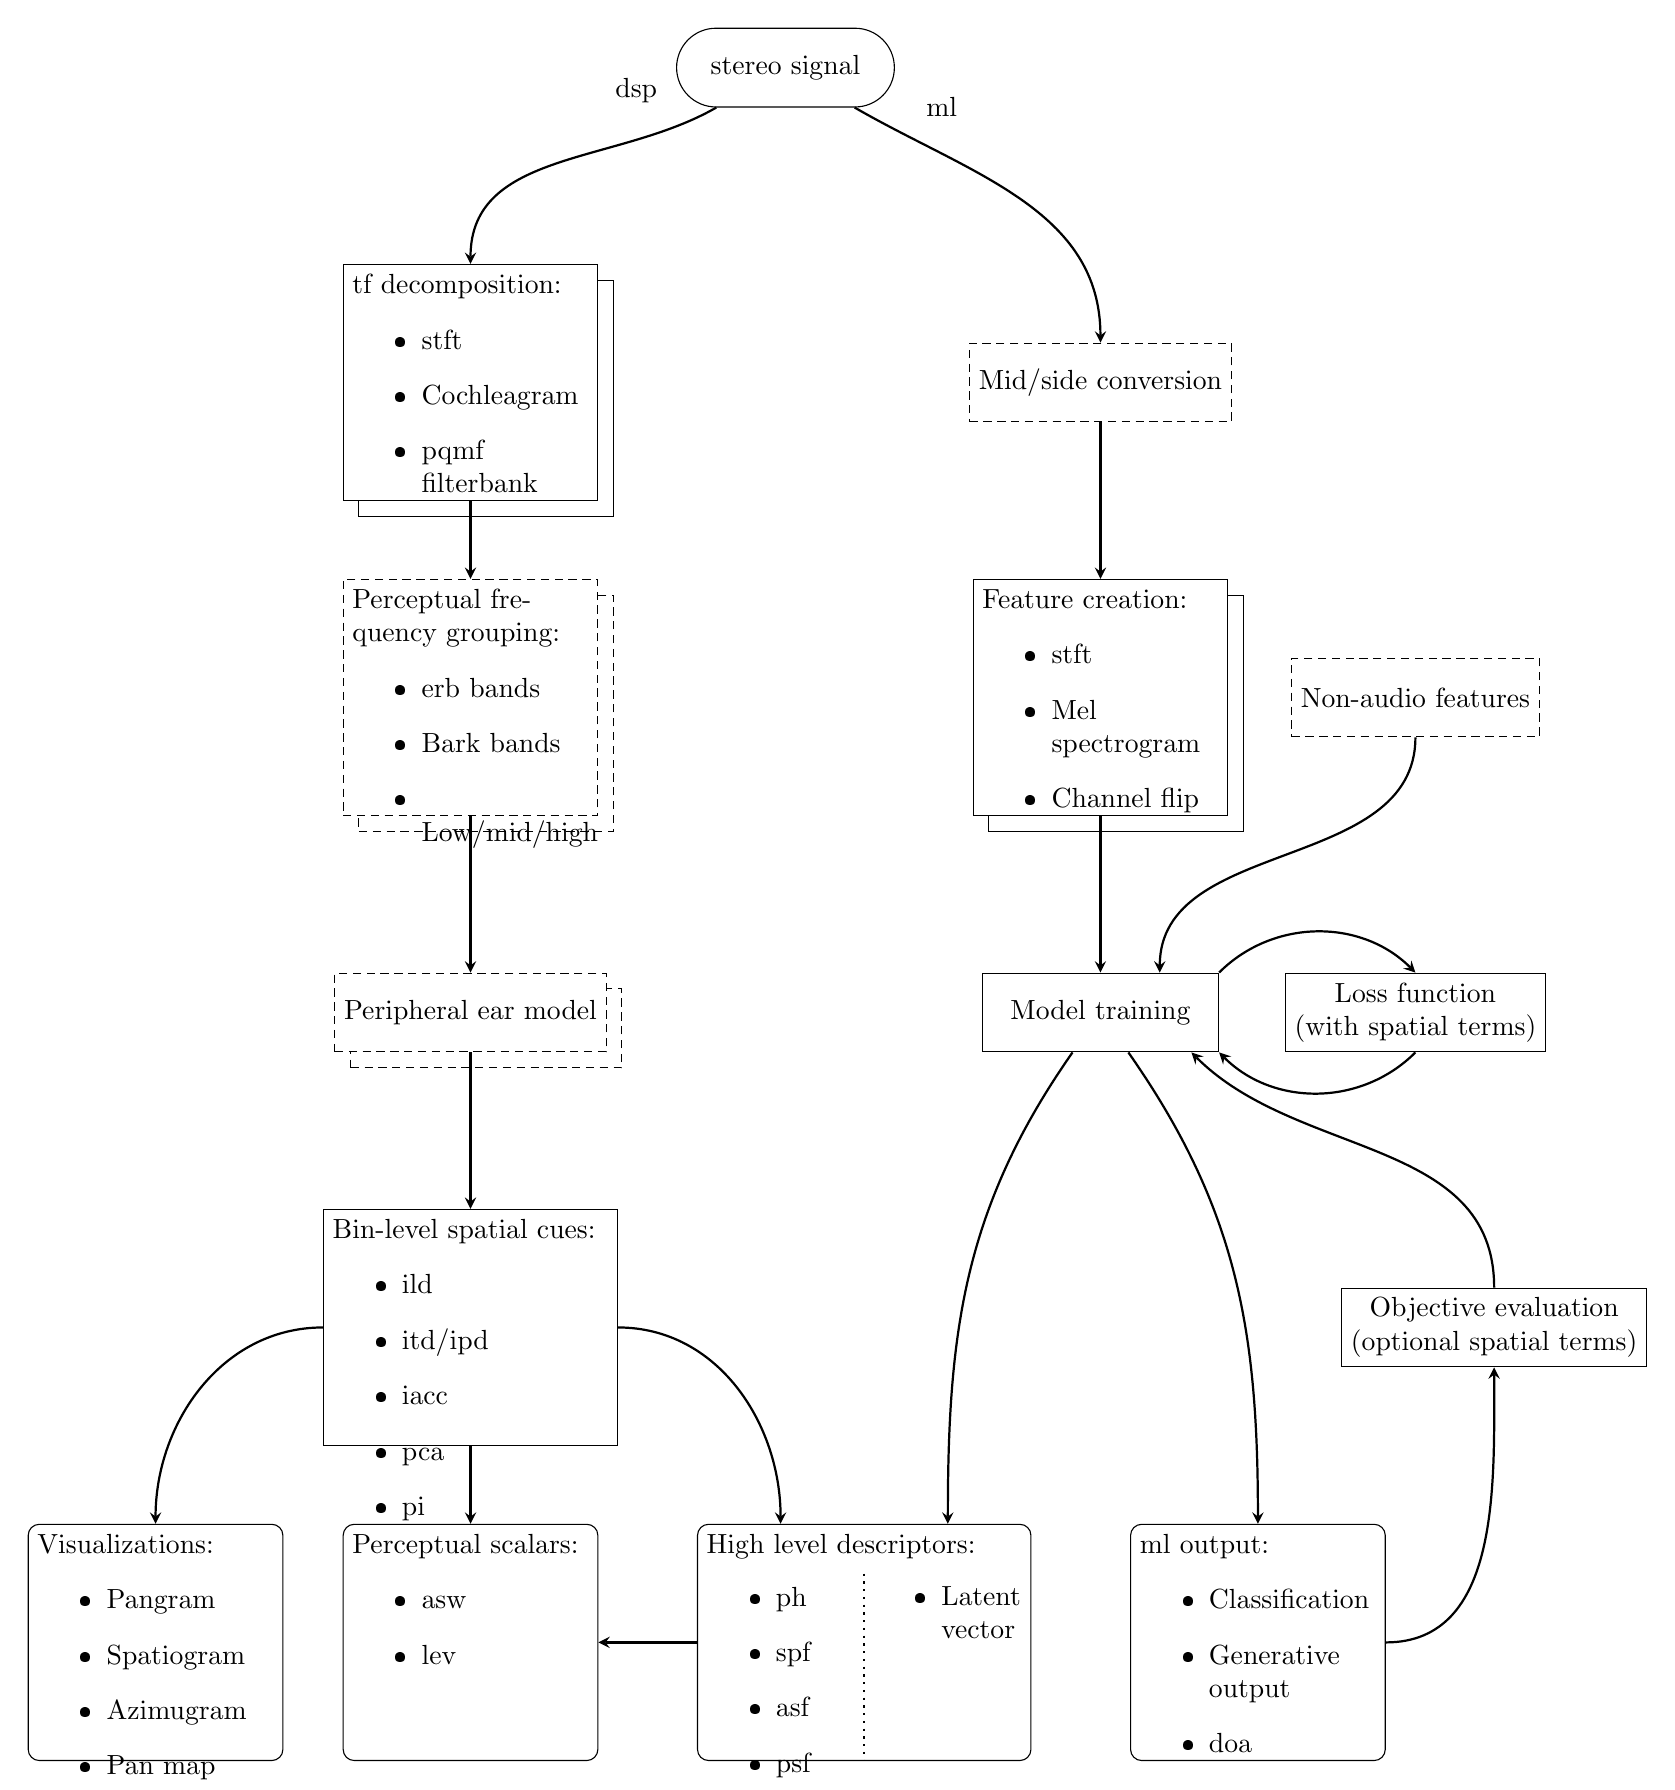
\begin{tikzpicture}[>=latex, node distance=4cm]

  \tikzstyle{textrect} = [rectangle, minimum width=3cm, minimum height=1cm, draw=black, fill=white, align=center]
  \tikzstyle{list} = [text depth=2.5cm, minimum height=3cm, text width=3cm, align=left]
  \tikzstyle{input} = [rounded rectangle, minimum width=3cm, minimum height=1cm, draw=black]
  \tikzstyle{arrow} = [thick,->,>=stealth]
  \tikzstyle{stereo} = [copy shadow={shadow xshift=0.2cm,shadow yshift=-0.2cm}]
  \tikzstyle{output} = [rounded corners]
  \tikzstyle{optional} = [densely dashed]
  \tikzstyle{path label} = [above, near start, outer sep = 1em]

  % Audio input
  \node[input] (audio) {stereo signal};

  % DSP path
  \node[textrect,stereo,list] (tfd) [below of=audio, xshift=-4cm] { \gls{tf} decomposition:
    \begin{itemize}
      \item \gls{stft}
      \item Cochleagram
      \item \gls{pqmf} filterbank
    \end{itemize}
  };
  \node[textrect,stereo,list,optional] (pg) [below of=tfd] {Perceptual frequency grouping:
    \begin{itemize}
      \item \gls{erb} bands
      \item Bark bands
      \item Low/mid/high
    \end{itemize}
  };
  \node[textrect,stereo,optional] (pem) [below of=pg] {Peripheral ear model};
  \node[textrect,list,text width=3.5cm] (bin) [below of=pem] {Bin-level spatial cues:
    \begin{itemize}
      \item \gls{ild}
      \item \gls{itd}/\gls{ipd}
      \item \gls{iacc}
      \item \gls{pca}
      \item \gls{pi}
    \end{itemize}};
  \node[textrect,output,list] (viz) [below of=bin, xshift=-4cm] {Visualizations:
    \begin{itemize}
      \item Pangram
      \item Spatiogram
      \item Azimugram
      \item Pan map
    \end{itemize}
  };
  \node[textrect,output,list] (ps) [below of=bin] {Perceptual scalars:
    \begin{itemize}
      \item \gls{asw}
      \item \gls{lev}
    \end{itemize}
  };
  \node[textrect,output,list] (hld) [below of=bin, xshift=5cm, text width=4cm] {High level descriptors:
  \begin{minipage}[t]{2.1cm}
    \vspace{0pt}
    \begin{itemize}
      \item \gls{ph}
      \item \gls{spf}
      \item \gls{asf}
      \item \gls{psf}
    \end{itemize}
  \end{minipage}%
  \begin{minipage}[t]{1.9cm}
    \vspace{0pt}
    \begin{itemize}
      \item Latent vector
    \end{itemize}
  \end{minipage}
  };

  % ML path
  \node[textrect,optional] (ms) [below of=audio, xshift=4cm] {Mid/side conversion};
  \node[textrect,stereo,list] (fc) [below of=ms] {Feature creation:
    \begin{itemize}
      \item \gls{stft}
      \item Mel spectrogram
      \item Channel flip
    \end{itemize}
  };
  \node[textrect,optional] (naf) [right of=fc] {Non-audio features};
  \node[textrect] (ml) [below of=fc] {Model training};
  \node[textrect,output,list] (mlout) [below of=ml, yshift=-4cm, xshift=2cm] {\gls{ml} output:
    \begin{itemize}
      \item Classification
      \item Generative output
      \item \gls{doa}
    \end{itemize}
  };
  \node[textrect] (loss) [right of=ml] {Loss function \\ (with spatial terms)};
  \node[textrect] (obj) [right of=mlout, yshift=4cm, xshift=-1cm] {Objective evaluation \\ (optional spatial terms)};

  % DSP edges
  \draw[arrow] (audio) to [out=210,in=90] node [path label] {\gls{dsp}} (tfd);
  \draw[arrow] (tfd) -- (pg);
  \draw[arrow] (pg) -- (pem);
  \draw[arrow] (pem) -- (bin);
  \draw[arrow] (bin) to [out=180,in=90] (viz.north);
  \draw[arrow] (bin) -- (ps);
  \draw[arrow] (bin) to [out=0,in=90] ($(hld.north west)!0.5!(hld.north)$);
  \draw[arrow] (hld) -- (ps);

  % ML edges
  \draw[arrow] (audio) to [out=330,in=90] node [path label] {\gls{ml}} (ms);
  \draw[arrow] (ms) -- (fc);
  \draw[arrow] (fc) -- (ml);
  \draw[arrow] (naf.south) to [out=270,in=90] ($(ml.north)!0.5!(ml.north east)$);
  \draw[arrow] (ml) to [out=235,in=90] ($(hld.north)!0.5!(hld.north east)$);
  \draw[arrow] (ml) to [out=305,in=90] (mlout.north);
  \draw[arrow] (ml.north east) to [out=45,in=135] (loss.north);
  \draw[arrow] (loss.south) to [out=225,in=-45] (ml.south east);
  \draw[arrow] (mlout.east) to [out=0,in=270] (obj.south);
  \draw[arrow] (obj.north) to [out=90,in=-45] ([xshift=-1em]ml.south east);

  % High level descriptor divider line
  \draw[dotted, thick] ([yshift=-1.8em]hld.north) -- (hld.south) {};

  \end{tikzpicture}
}

\end{figure}

Although not shown on the diagram, it is important to choose spatial features that are relevant for the type of input audio and the intended output features. For example, if the input is standard stereophonic music and the output is intended to convey amplitude panning, then all phase-based spatial cues can be eliminated. However, if the output is intended to show \gls{lev} (even given the same stereophonic input), then phase cues cannot be eliminated. If the input audio is binaural, both phase and amplitude differences are relevant, but the frequency bands in which they are relevant differ depending on the intended output. E.g. \gls{doa} only requires phase below approximately 1500Hz \cite{morinagaEvaluationMethodCoded}, but other tasks should follow a binaural hearing model with more complex frequency weighting \cite{schaferExtensionPEAQMeasure2013,nowakQualityAssessmentSpherical2019}.


\subsection{Validation techniques}
\label{sec:validation_techniques}

The papers surfaced in this review revealed several high-level categories of techniques to validate the success of the research. They tend to be closely linked to the downstream task, although some are universal. The most prevalent were perceptual listening tests, used in approximately half the studies. Some standardized perceptual tests are ITU-R-BS.1534 \cite{itu-r-bs-1534_MUSHRA}, which defines the \gls{mushra} test used for measuring \q{intermediate audio quality}, and ITU-R-BS.1116 \cite{itu-r-bs.1116-1MethodsSubjectiveAssessment1997} which is used for measuring \q{small impairments} in audio quality. In general though, it is more common to set up a custom subjective test asking the participants directly about the audio feature of interest. Several studies \cite{gunnarssonSpectralCorrectionAudio2024,gunnarssonPracticalMethodHRTF2022,madmoniEffectPartialTimeFrequency2021,arthisSpatiogramPhaseBased2021} described their subjective tests as \q{\glsxtrshort{mushra}-like}, showing that the standardized frameworks are useful as a basis even if they don't perform the exact task required.

The second popular validation technique is objective metrics. The studies reviewed used a large variety of different metrics, although there is some standardization within specific scientific communities. For example, the \gls{bsseval} software library is frequently used to measure the similarity of audio waveforms in source separation tasks \cite{vincentPerformanceMeasurementBlind2006}. The same library can also be used for any task where waveform similarity is pertinent, e.g. \cite{wuStackedSparseAutoencoder2021} which is concerned with audio coding and compression. Another option for comparing the similarity of two waveforms is the \q{spectrogram difference} \cite{hsuModelMatchingPrincipleApplied2023}, which can be considered more in line with human perception but naturally contains a trade-off in time and frequency resolution. Of note here is that the aforementioned techniques are tailored towards monophonic audio (although they can trivially be extended to multiple channels). More specific comparison metrics such as \gls{psd} \cite{armstrongPerceptualSpectralDifference2018} or \gls{bamq} \cite{flessnerAssessmentPredictionBinaural2017} can be used to describe the difference between two stereo (specifically, binaural) signals. For perceptual differences in higher audio models (e.g. multichannel or ambisonics) it is typical to record or render the audio to a binaural signal and evaluate that \cite{choiObjectiveMeasurementPerceived2008,kiyanPredictingImmersionSurround2023,stahlPerceptualComparisonParametric2023}.

If the research in question is related to creating or testing an objective metric, it can be useful to reverse the problem; One can perform simulations of real audio data by designing a set of signals with predictable differences, and analyse the results of the metric. \cite{watcharasupatQuantifyingSpatialAudio2024} is one such example in which a novel metric is defined, and then its real results are tested against theoretical ones. In addition, diagrams are of the simulations are shown for visual inspection. This is another common validation technique in studies where a known, correct, low-dimensional value can be compared against a higher-dimensional metric, e.g. \cite{takanenBinauralAuditoryModel2012} which compares the panning position of an instrument to the peak in a \gls{ph}, or \cite{lluisDeepLearningApproach2022} which compares a known azimuth and elevation with various activity maps generated from ambisonic audio. Note that comparing the similarity of \glspl{ph} is error-prone as the standard distance metrics (e.g. Euclidean distance) don't necessarily correlate with perceptual difference \cite{miticObjectiveComparisonPanning2025}. \cite{gomezMusicSimilaritySystems2008} attempts to side-step this issue by converting \glspl{ph} into a different domain, although the efficacy of this approach remains largely unexplored.


In the \gls{ml}/\gls{dl} sphere it is normal to calculate the success of a model by its percentage of correct predictions, both for classical \gls{ml} \cite{tzanetakisStereoPanningFeatures2007,tardieuProductionEffectAudio2011,chenMixedStereoAudio2014}, and more modern \gls{dl} approaches \cite{zielinskiAutomaticDiscriminationFront2022,zielinskiImprovingClassificationBasic2020,zielinskiSpatialAudioScene2022}. However, this obviously only works with labelled data. In the case that labels don't exist, one option is to create a self-supervised \q{pretext task} in which labelled data can be generated from unlabelled \cite{yangSelfSupervisedLearningSpatial2024,satoSelfSupervisedLearningAudioVisual2022,mourgelaExploringTrendsAudio2024,liCrossmodalGenerativeModel2024}. In cases where there are no known objective metrics for the task at hand (e.g. the plausibility of novel stereo renderings \cite{serraMonotostereoParametricStereo2023}) inspiration can be taken from non-audio-domain tasks, utilizing e.g. the minimum error of a large sample or the Fréchet distance between real and generated parameter spaces \cite{tomczakDeepGenerativeModeling2024}.

An under-studied but nonetheless important metric is the computational complexity of the algorithm described. Typical metrics to measure this are the time taken to process a given duration of audio on specific hardware \cite{gorlowInformedSeparationSpatial2013}, number of \glspl{flop} \cite{zhuEndtoEndPairedAmbisonicBinaural2024}, or (for \gls{ml}/\gls{dl}) number of network parameters \cite{zhuEndtoEndPairedAmbisonicBinaural2024}.


\subsection{Audio datasets}
\label{sec:audio_datasets}

\subsubsection{Existing datasets}
\label{sec:existing_audio_datasets}
\Cref{tab:audio_datasets} shows a comprehensive list of audio datasets that were referenced by papers in this review. The only exception is \q{mobygratis} \cite{MobygratisFreeMoby2025}, which was released after the review was performed but nonetheless presents similar opportunities for research. Datasets that were not available publicly such as those used in \gls{mpeg} standardization have been omitted, and the availability of each dataset is noted. The \q{Size} column represents the number of musical tracks or clips present in the dataset, but does not take their lengths into account. Non-musical recordings are not counted. Since it is assumed that larger and more varied datasets are preferable, the table is ordered by \q{Size}. The columns \q{M}, \q{S}, and \q{B} indicated whether the datasets contain multitrack\footnote{A Multitrack recording indicates that individual stems of a recording session are available, but not necessarily a stereo mix.}, stereo, or binaural recordings respectively. \cite{IEEESignalProcessing2025,liCreatingMultitrackClassical2019,bogdanovMTGJamendoDatasetAutomatic2019} also contain lists of audio datasets (with some overlap to those listed here) that might be useful for future research.

\begin{sidewaystable}[htbp]
\caption{
Audio datasets, ordered by size (number of tracks or clips). \\
{\footnotesize
M=Multitrack, S=Stereo, B=Binaural\\
\textsuperscript{$\star$}Individual tracks. \textsuperscript{$\dagger$}Individual files. \textsuperscript{$\ddagger$}Must request access. \textsuperscript{$\S$}Exact size unclear.}
}
\label{tab:audio_datasets}
\setlength{\tabcolsep}{0.25em}
\begin{tabularx}{\textheight}{llllllllX}
\toprule
Name & Audio format & Size & Duration & M & S & B & Availability & Notes \\
\midrule
\glsxtrshort{fma}\cite{defferrardFMADatasetMusic2017} & mp3 various bitrates & 106574 & 343d &  & \checkmark &  & Download & Real music. Huge variety. Contains common audio features and tags. \\
\glsxtrshort{mtgj}\cite{bogdanovMTGJamendoDatasetAutomatic2019} & mp3 320kbps & 55609 & 157d &  & \checkmark &  & Download & Real music. Wide variety of genres, instruments, and moods. \\
ccMixter\cite{CcMixter} & Various mp3/wav & $\approx 48000$\textsuperscript{$\S$} & ?\textsuperscript{$\S$} & \checkmark & \checkmark &  & Download\textsuperscript{$\dagger$} & Real music in many genres. Some stereo, some stems. Vast, but some download links are broken. \\
\glsxtrshort{asascbrm}\cite{zielinskiDatabaseAutomaticSpatial2019} & wav 48kHz 24bit  & 5928 & 11h &  &  & \checkmark & Download & Synthesized binaural from other multitrack datasets. 30s clips. \\
Slakh\cite{manilowCuttingMusicSource2019} & wav 44.1kHz & 2100 & 145h & \checkmark & \checkmark &  & Download & Mono stems. Synthesized from midi. \\
FAIR-Play\cite{gao25DVisualSound2019} & wav 48kHz 16bit  & 1871 & 5h &  &  & \checkmark & Download & Binaural. 10s clips. Only 1 recording room. \\
\glsxtrshort{maestro}\cite{hawthorneEnablingFactorizedPiano2019} & wav 44.1/48kHz 16bit & 1276 & 199h &  & \checkmark &  & Download & Only classical piano \\
\glsxtrshort{msss}\cite{MixingSecretsFree} & wav 44.1kHz 16/24bit  & 625 & 40h & \checkmark & \checkmark &  & Download\textsuperscript{$\star$} & Stems uncompressed. Example stereo mixes in mp3 only \\
mobygratis\cite{MobygratisFreeMoby2025} & wav 44.1kHz 24bit & 499 & 35h & \checkmark & \checkmark &  & Download\textsuperscript{$\star$} & Stereo stems and mixdowns. Multiple genres but only 1 artist. \\
\glsxtrshort{rwc}\cite{gotoDevelopmentRWCMusic2004,gotoRWCMusicDatabase2002,gotoRWCMusicDatabase2003,gotoRWCMusicDatabase2012} & CD, 44.1kHz 16bit & 465 & 22h &  & \checkmark &  & CD\textsuperscript{$\ddagger$} & Multiple datasets each of a different genre \\
MedleyDB 2.0\cite{bittnerMedleyDB20New2016} & wav 44.1kHz 16bit & 330 & 7h & \checkmark &  &  & Download\textsuperscript{$\ddagger$} & Real music. Mix of genres. Some instrumental, some vocal. More tracks have been added since publication. \\
MUSDB18\cite{rafiiMUSDB18CorpusMusic2017} & AAC 256kbps & 150 & 10h & \checkmark &  &  & Download & Only stems. Derived from other datasets such as \cite{liutkus2016SignalSeparation2017,bittnerMedleyDBMULTITRACKDATASET2014} \\
MUSDB18-HQ\cite{rafiiMUSDB18HQUncompressedVersion2019} & wav 44.1kHz & 150 & 10h & \checkmark &  &  & Download & Only stems. Derived from other datasets such as \cite{liutkus2016SignalSeparation2017,bittnerMedleyDBMULTITRACKDATASET2014} \\
MedleyDB\cite{bittnerMedleyDBMULTITRACKDATASET2014} & wav 44.1kHz 16bit  & 132 & 7h & \checkmark &  &  & Download\textsuperscript{$\ddagger$} & Stereo mix + dry and processed stems \\
\glsxtrshort{dsd100}\cite{liutkus2016SignalSeparation2017} & wav 44.1khz & 100 & 7h & \checkmark & \checkmark &  & Download & Stems and downmixes, derived from \cite{MixingSecretsFree} \\
\glsxtrshort{btpab}\cite{zhuAmbisonicBinaural2022} & wav 48kHz 16bit  & 49 & 49m &  &  & \checkmark & Download & 60s clips. Only 1 recording session. \\
FiloSax\cite{fosterFilosax2021,fosterFilosaxDatasetAnnotated2021} & wav 44.1kHz 24bit & 48 & 5h & \checkmark &  &  & Download\textsuperscript{$\ddagger$} & Only jazz \\
\glsxtrshort{daoc}\cite{variousAnechoicOrchestralMusic1988} & CD, 44.1kHz 16bit & 44 & 25m &  & \checkmark &  & CD & Anechoic orchestra \\
\glsxtrshort{urmp}\cite{liCreatingMultitrackClassical2019} & wav 48kHz 24bit  & 44 & 1h & \checkmark &  &  & Download & Anechoic classical music. Only stems. \\
\glsxtrshort{boma}\cite{bangolufsenMusicArchimedes1992,hansenMakingRecordingsSimulation1991} & CD, 44.1kHz 16bit & 31 & 1h &  & \checkmark & \checkmark & CD & Anechoic and semi-reverberant orchestra. \\
\glsxtrshort{tss}\cite{MultitracksTelefunkenElektroakustik2022} & wav 44.1kHz 16bit & 23 &  & \checkmark &  &  & Download\textsuperscript{$\star$} & Both live and studio sessions. \\
\glsxtrshort{quasi}\cite{fillonQUASIDatabaseMusical2012} & wav 44.1kHz & 11 & $\approx 30m$\textsuperscript{$\S$} & \checkmark &  &  & Download\textsuperscript{$\ddagger$} & Mix of genres \\
\glsxtrshort{sqam}\cite{UsersHandbookEBU2008} & FLAC 44.1kHz 16bit & 10 & 1h &  & \checkmark &  & Download & Not all music, some stereo some mono. \\
\glsxtrshort{rioossr}\cite{dorazioRecordingsItalianOpera2016} & wav 48kHz 24bit & 4 & 5m &  &  &  & Download & Ambisonic and channel-based versions \\
\glsxtrshort{arsso}\cite{patynenAnechoicRecordingSystem2008} & mp3 192kbps 48kHz & 4 & 11m & \checkmark &  &  & \thead[l]{\scalebox{.8}[1.0]{mp3: Download}\\\scalebox{.8}[1.0]{wav: Contact author}} & Anechoic classical music. Only stems. \\
\glsxtrshort{uiowamis}\cite{UniversityIowaMusical} & \thead[l]{wav 44.1kHz 16bit\\ or 96kHz 24bit} & ?\textsuperscript{$\S$} & 23h &  & \checkmark &  & Download\textsuperscript{$\dagger$} & Individual notes. Approximately 85\% stereo, 15\% mono. \\
Bach10\cite{duanMultipleFundamentalFrequency2010} & wav 44.1kHz & ?\textsuperscript{$\S$} & ?\textsuperscript{$\S$} &  &  &  & Contact author & Only Bach chorales. \\
\bottomrule
\end{tabularx}

\end{sidewaystable}


\subsubsection{Synthesized datasets}
\label{sec:synthesized_audio_datasets}
It is often the case than a dataset matching the exact task at hand does not exist, in which case one is synthesized from other datasets. In fact, some datasets listed in \cref{tab:audio_datasets} are amalgamations of others -- see the \q{Notes} column for details.

When creating a custom dataset, the most prevalent technique surfaced in this review was to convolve monophonic audio with some form of \gls{ir}. Said \gls{ir} can be binaural (e.g. \cite{nastasiPsychoAcousticalExperimentUsing2020}), ambisonic (e.g. \cite{lluisDirectionSpecificAmbisonics2023}), or a microphone array (e.g. \cite{coteliSphericalHarmonicsBased2021}). It is also common that these the \glspl{ir} add reverberation to a recording, as in e.g. \cite{uhleSubbandCenterScaling2014,coteliMultipleSoundSource2019,tylerPredictingBinauralRoom2023,gerkenComparison2D3D2024}. For research focused on binaural audio, \cite{zielinskiAutomaticDiscriminationFront2022} contains a comprehensive list of publicly available \gls{hrir} datasets.

Synthetic datasets of stereo music are slightly different in that they must be manually mixed from monophonic stems, which can be amplitude-panned in any way that the experiment requires. E.g. in \cite{harmaStereoAudioClassification2011} the stems are placed according to the signal model described in the study, and \cite{petermannSpainNetSpatiallyInformedStereophonic2022,yangUpmixingStyleTransfer2022} pan the stems randomly.

Taking a slightly different route, \cite{manilowCuttingMusicSource2019} introduces a dataset of song stems synthesized entirely from \gls{midi} files using professional-grade \glspl{vi}, motivated by a lack of commercial music datasets offering stems.


\subsection{Uses of \glsxtrlongpl{sip}}
\label{sec:uses_of_sips}

\subsubsection{Current uses}
\label{sec:current_uses_of_sips}

Broadly speaking, there are two categories of tasks that spatial information in audio has historically been used for. Firstly there are those focused on a single recording from which the information was extracted. Compression, source separation and upmixing are the most prevalent examples which arose in this review. In recent years, these have become somewhat intertwined with the advent of new commercial spatial audio formats such as Dolby Atmos and MPEG-H 3D Audio; older content which was released in stereophonic or multichannel format can benefit from combinations of source separation, upmix, and coding/compression techniques that increase the perceptual quality when rendered on modern equipment. The spatial attributes extracted in these cases tend to be the low-level spatial cues detailed in \cref{sec:binaural_and_spatial_cues} since the tasks naturally require that the original audio is re-synthesized in some way.

Quality prediction (and in particular, \textit{spatial} quality prediction) is another area of considerable interest, the driving force being that traditional perceptual listening tests are slow and costly \cite{engelAssessingHRTFPreprocessing2022,delgadoDesignChoicesBinaural2023}. This differs slightly from the previously mentioned tasks in that it implies a comparison between a reference and degraded signal, and uses summaries of low-level spatial cues combined with non-spatial measurements.  The type of spatial attributes used in these cases are more in line with the high-level descriptors detailed in \cref{sec:high_level_descriptors}. In particular, \cite{choiPredictionPerceivedQuality2007,choiObjectiveMeasurementPerceived2008,youSpatialLocalizationEvaluation2012,watcharasupatQuantifyingSpatialAudio2024} use distortion/difference of \gls{ild}/\gls{itd}/\gls{itd} in their perceptual models, and \cite{supperOnsetGuidedSpatialAnalyser2005,dewhirstModellingPerceivedSpatial2008} use \q{sound field maps} or \glsxtrlongpl{ph} to describe the spatial information present in the analysed audio. Combining the two approaches, \cite{delgadoObjectiveAssessmentSpatial2019} defines the \gls{dsd} metric to show the difference between a reference and degraded \q{directional loudness map}.

The studies surfaced in this review reveal that there was a spike of interest in binaural quality prediction and analysis since 2023. This appears to be driven by a renewed interest in spatial audio\footnote{As mentioned in \cref{sec:validation_techniques}, the typical way to measure perceptual effects of higher-order audio models is to render them to a binaural signal.} \cite{delgadoDesignChoicesBinaural2023,stahlPerceptualComparisonParametric2023,pfanzagl-cardoneArtScience3D2023,bergnerIdentificationDiscriminativeAcoustic2023,kiyanPredictingImmersionSurround2023}, room acoustics \cite{tylerPredictingBinauralRoom2023,vonbergAnalysisPhysicalPerceptual2024} and \gls{vr} rendering \cite{marchanMultiLayeredArchitectureEfficient2023,politisWideArea6DOFRendering2023,yeLAVSSLocationGuidedAudioVisual2024}, along with the increased ease of gathering or creating binaural audio datasets.

Secondly, there are those tasks which focus on the relationship of a single recording to a larger corpus. Classification is a typical use case, with the list of predicted labels including genre/recording style \cite{tzanetakisStereoPanningFeatures2007,tzanetakisStereoPanningInformation2010,ziemerGoniometersArePowerful2023}, artist/composer/\glsxtrshort{dj} \cite{tzanetakisStereoPanningInformation2010,ziemerAcousticFeaturesRecording2021}, and decade \cite{tardieuProductionEffectAudio2011}. Important to note in all of these cases is that the ground truth is known a-priori. However, with the vast size of modern audio datasets, acquiring reliable annotations becomes increasingly difficult. For example, \cite{colonelReverseEngineeringRecording2021,rodriguezSpectralDynamicConstellations2024} both specifically state that panning parameters, \gls{daw} sessions, and musical scores are typically not available for most recorded music, and therefore any such information must be derived after-the-fact from a mixdown.

An interesting middle-ground between the two categories can be found in the aforementioned \cite{barryMusicStructureSegmentation2007}, which uses temporal changes in \glspl{ph} to segment a song into musical structures (verse, chorus, etc.). Likewise, \cite{harmaClassificationTimefrequencyRegions2011,harmaStereoAudioClassification2011} attempt both a generic classification of stereo field, and a further application to segment longer audio recordings using that classifier.

In addition, a frequently occurring pattern among studies in this review is that spatial cues are used as objective measurements for other tasks. In particular, \cite{erruzBinauralSourceSeparation2017,zhuAmbisonicBinaural2022,limEnhancingSpatialAudio2024} demonstrate that the incorporation of spatial terms into \gls{dl} loss functions, forcing the networks to learn or generate spatial features.


\subsubsection{Potential uses}
\label{sec:potential_uses_of_sips}
Compelling areas for further research can be inferred from what is missing from the survey results. In total, 41 studies were deemed to be making use of \gls{ml} or \gls{dl}, all of which were performing some form of \textit{supervised} learning. Just a single study \cite{ziemerGoniometersArePowerful2023} mentioned performing \textit{unsupervised} learning on spatial cues --- a self-organising map was used to discriminate between two clusters of tracks when simple linear regression failed. \cite{wangUnsupervisedDeepLearning2020} presents a similar study, although the audio was non-musical. \cite{miticObjectiveComparisonPanning2025} gives an overview of the suitability of various panning feature with regard to unsupervised learning, and \cite{barryBinaspectPythonLibrary2025} describes some spatial cues that can be used as input to \gls{ml} routines. (Notably, both emerged after the database search for this review was performed).

Likewise, relatively few studies perform any spatial analysis of extremely large and varied musical datasets. E.g. \cite{hsuModelMatchingPrincipleApplied2023} used music clips from \gls{fma}\cite{defferrardFMADatasetMusic2017} as background noise in a task focused on the binaural rendering of speech, and while the standard spatial cues were extracted, the music was not of primary interest. \cite{tzanetakisStereoPanningFeatures2007,tzanetakisStereoPanningInformation2010,tardieuProductionEffectAudio2011} use mid-size (thousands of tracks) datasets to demonstrate various classification tasks, although they unfortunately predate the existence of the aforementioned extremely large datasets. Nonetheless, these older studies present an interest in the dataset itself as opposed to low-level features of the audio. A much more recent study \cite{mourgelaExploringTrendsAudio2024} expresses a similar interest, measuring production tends in a huge (albeit private) dataset containing hundreds of thousands of tracks. Analysis of the spatial features in vast musical corpora therefore presents an opportunity for further research. In particular, there are no studies on spatial degradation caused by lossy compression of said datasets, even though the largest \cite{defferrardFMADatasetMusic2017,bogdanovMTGJamendoDatasetAutomatic2019} are both encoded using the \gls{mp3} codec, and \cite{barryBinaspectPythonLibrary2025} clearly shows the effects of lossy compression on the \gls{ild} and \gls{itd} of their test signals.

\cite{ziemerUsingPsychoacousticModels2016,wilsonPerceptionAudioQuality2016} present a further basis for investigation, concluding that two objective measures of spaciousness (\gls{iccc} and \gls{spf}) did not match the results of a perceptual music similarity test. This issue warrants further investigation, since research into the \glspl{sip} of tracks in a large music corpus will naturally involve a measure of similarity.


\section{Discussion}
\label{sec:discussion}

Overall, this review paints a picture of a research landscape that is somewhat fractured. The core psychoacoustic principals and terminology is fairly well standardized, although many researchers offer their own variations on the precise implementations and inferences of both high-level spatial features and low-level spatial cues. The net result is that searching for relevant literature by \textit{downstream task} rather than by rather than \textit{spatial attribute} will usually be most efficient. However, this method presents diminishing returns for tasks with few previous examples or non-standard terminology (such as finding \glspl{sip}), and the opportunity of \q{cross-pollination} from other fields of audio research is lost. This review intended to fix the cross-pollination problem, although it turned out that the resulting scope was so large as to effectively limit the usefulness of a human reviewer. Experiments in performing audio-related literature reviews using \glspl{llm} have shown potential, although it was concluded that they are no substitute for human researchers \cite{santosExploringPotentialDataDriven2024}.

Open-source tooling such as those mentioned in \cref{sec:standard_spatial_cues} go some way to towards giving researchers a shared language around spatial aspects of stereo audio. Indeed, many of the studies in this review contained links to both source code and sound samples, but precious few were still active. The move towards shared audio datasets is a step forward though, since until recently large datasets of real music were either completely unavailable or confined to private collections. With the introduction of the datasets listed in \cref{sec:audio_datasets} it might now be possible for music-specific audio research to share a common footing, just as happened in the image processing community \cite{defferrardFMADatasetMusic2017}.

While this review aimed to provide an exhaustive list of spatial descriptors, the fact that some studies were only added after following references shows that the original search method was not foolproof. Similarly, since there were several papers added by recommendations after the initial search took place, it is a sign that there is renewed interest of spatial features within the audio research community, likely resulting in a pool of relevant studies that could not have been captured.

\section{Conclusion}
\label{sec:conclusion}

A \glsxtrfull{slr} following the \gls{prisma} guidelines was performed to find methods of describing the \glsxtrfull{sip} of stereophonic music recordings. The terminology, methods, and signal processing techniques are listed in detail, and the conglomeration of data extracted from the included studies provides a framework from which custom \gls{sip} algorithms appropriate for any given task can be designed and implemented. Datasets containing suitable audio material are also listed alongside descriptions of the contained audio.

While the focus was on stereophonic recordings, many studies are equally relevant to other audio formats such as multichannel and ambisonics. Readers can benefit from inspiration and \q{cross pollination} of diverse areas of audio research, and the review as a whole enables researchers and practitioners to jump-start new studies into the spatial aspects of music.


\printglossaries



\backmatter

% \bmhead{Supplementary information}

% If your article has accompanying supplementary file/s please state so here.


\section*{Declarations}

\subsection{Availability of data and materials}
The dataset supporting the conclusions of this article is included as an additional file. It comprises a concatenation of search results from the three databases searched, in \gls{csv} format. The columns are:

\begin{table}[htbp]
  \centering
  \caption{Explanation of fields in accompanying file of database search results}
  \begin{tabularx}{\textwidth}{lX}
    \toprule
    Header & Explanation \\
    \midrule
    \verb|url|             & The \gls{url} of the record within the database \\
    \verb|title|           & The title of the article \\
    \verb|abstract|        & The abstract of the article \\
    \verb|year|            & The year of publication \\
    \verb|authors|         & The authors of the article, in the raw format given by the search results \\
    \verb|source|          & The publication venue \\
    \verb|DOI|             & The \gls{doi} of the article \\
    \verb|citation_count|  & The number of citations recorded within the specific database \\
    \verb|db|              & The name of the database from which the record was extracted \\
    \verb|db_id|           & The unique ID number within the database \\
    \bottomrule
  \end{tabularx}
  \label{tab:search_results_csv}
\end{table}

\subsection{Competing interests}
The author declared that they have no competing interests.

\subsection{Funding}
This research was funded in part by \gls{kks} -- \href{https://kks.se}{https://kks.se}.

\subsection{Ethics approval and consent to participate}
Not applicable

\subsection{Author contribution}
RM is the sole author.

\subsection{Acknowledgements}
Not applicable

\subsection{Author Info}
RM is a doctoral candidate at M{\"a}lardalen University, currently researching spatial audio, digital signal processing, and large-scale \gls{mir}. He holds a master's degree in Music and Electronics from the University of Glasgow where he specialized in digital electronics and audio processing. He has spent many years working in industry, starting as a researcher of media streaming protocols and participating in \gls{mpeg} standardization, later progressing into the music industry where he wrote software for music streaming, media transcoding, real-time audio, and embedded devices.


\begin{appendices}

\section{Search terms}
\label{ap:search_terms}
\noindent \textbf{Population}: \enquote{music},\enquote{musical},\enquote{audio},\enquote{sound}

\noindent \textbf{Context}: \enquote{stereo}, \enquote{stereophonic}, \enquote{binaural}, \enquote{spatial audio}, \enquote{ambisonic}, \enquote{ambisonics}, \enquote{b-format}, \enquote{multi-channel}

\noindent \textbf{Outcome}: \enquote{panning}, \enquote{information retrieval}, \enquote{spaciousness}, \enquote{descriptors}, \enquote{spatial image}, \enquote{stereo image}, \enquote{spatial cues}, \enquote{disentangle}, \enquote{disentangling}, \enquote{disentanglement}, \enquote{spatial decomposition}, \enquote{spatial information}, \enquote{spatial descriptors}, \enquote{spatial quality}, \enquote{spatial analysis}, \enquote{binaural model}, \enquote{goniometer}, \enquote{lissajous plot}, \enquote{systematic review}

\noindent \textbf{Negative terms}: \enquote{stereo vision}, \enquote{computer vision}, \enquote{image processing}, \enquote{stereo camera}, \enquote{stereo cameras}

\noindent \textbf{Specific terms}: \enquote{spatial audio coding}, \enquote{spatial audio object coding}, \enquote{directional audio coding}, \enquote{binaural cue coding}, \enquote{panning spectrogram}, \enquote{stereo panning spectrum}, \enquote{object-based audio}, \enquote{mpeg-h audio}, \enquote{mpeg-h 3D audio}, \enquote{dolby atmos}, \enquote{sony 360 audio}, \enquote{sony 360 RA}, \enquote{360 reality audio}, \enquote{QESTRAL}

\section{Database Queries}
\label{app:database_queries}

\noindent\begin{minipage}{\linewidth}
\begin{singlespace}
\begin{lstlisting}[caption=Scopus query]
TITLE-ABS-KEY(((("music" OR "musical" OR "audio" OR "sound") AND ("stereo" OR "stereophonic" OR "binaural" OR "spatial audio" OR "ambisonic" OR "ambisonics" OR "b-format" OR "multi-channel") AND ("panning" OR "information retrieval" OR "spaciousness" OR "descriptors" OR "spatial image" OR "stereo image" OR "spatial cues" OR "disentangle" OR "disentangling" OR "disentanglement" OR "spatial decomposition" OR "spatial information" OR "spatial descriptors" OR "spatial quality" OR "spatial analysis" OR "binaural model" OR "goniometer" OR "lissajous plot" OR "systematic review")) AND NOT ("stereo vision" OR "computer vision" OR "image processing" OR "stereo camera" OR "stereo cameras")) OR ("spatial audio coding" OR "spatial audio object coding" OR "directional audio coding" OR "binaural cue coding" OR "panning spectrogram" OR "stereo panning spectrum" OR "object-based audio" OR "mpeg-h audio" OR "mpeg-h 3D audio" OR "dolby atmos" OR "sony 360 audio" OR "sony 360 RA" OR "360 reality audio" OR "QESTRAL"))
\end{lstlisting}
\end{singlespace}
\end{minipage}

\noindent\begin{minipage}{\linewidth}
\begin{singlespace}
\begin{lstlisting}[caption=\glsxtrlong{wos} query]
((((TS=("music") OR TS=("musical") OR TS=("audio") OR TS=("sound")) AND (TS=("stereo") OR TS=("stereophonic") OR TS=("binaural") OR TS=("spatial audio") OR TS=("ambisonic") OR TS=("ambisonics") OR TS=("b-format") OR TS=("multi-channel")) AND (TS=("panning") OR TS=("information retrieval") OR TS=("spaciousness") OR TS=("descriptors") OR TS=("spatial image") OR TS=("stereo image") OR TS=("spatial cues") OR TS=("disentangle") OR TS=("disentangling") OR TS=("disentanglement") OR TS=("spatial decomposition") OR TS=("spatial information") OR TS=("spatial descriptors") OR TS=("spatial quality") OR TS=("spatial analysis") OR TS=("binaural model") OR TS=("goniometer") OR TS=("lissajous plot") OR TS=("systematic review"))) NOT (TS=("stereo vision") OR TS=("computer vision") OR TS=("image processing") OR TS=("stereo camera") OR TS=("stereo cameras"))) OR (TS=("spatial audio coding") OR TS=("spatial audio object coding") OR TS=("directional audio coding") OR TS=("binaural cue coding") OR TS=("panning spectrogram") OR TS=("stereo panning spectrum") OR TS=("object-based audio") OR TS=("mpeg-h audio") OR TS=("mpeg-h 3D audio") OR TS=("dolby atmos") OR TS=("sony 360 audio") OR TS=("sony 360 RA") OR TS=("360 reality audio") OR TS=("QESTRAL")))
\end{lstlisting}
\end{singlespace}
\end{minipage}

\noindent\begin{minipage}{\linewidth}
\begin{singlespace}
\begin{lstlisting}[caption=\glsxtrlong{ss} query]
(("music" | "musical" | "audio" | "sound") + ("stereo" | "stereophonic" | "binaural" | "spatial audio" | "ambisonic" | "ambisonics" | "b-format" | "multi-channel") + ("panning" | "information retrieval" | "spaciousness" | "descriptors" | "spatial image" | "stereo image" | "spatial cues" | "disentangle" | "disentangling" | "disentanglement" | "spatial decomposition" | "spatial information" | "spatial descriptors" | "spatial quality" | "spatial analysis" | "binaural model" | "goniometer" | "lissajous plot" | "systematic review")) | ("spatial audio coding" | "spatial audio object coding" | "directional audio coding" | "binaural cue coding" | "panning spectrogram" | "stereo panning spectrum" | "object-based audio" | "mpeg-h audio" | "mpeg-h 3D audio" | "dolby atmos" | "sony 360 audio" | "sony 360 RA" | "360 reality audio" | "QESTRAL")
\end{lstlisting}
\end{singlespace}
\end{minipage}

\section{Semantic Scholar \gls{api} payload}
\noindent\begin{minipage}{\linewidth}
\begin{singlespace}
\begin{lstlisting}[
  caption=\gls{ss} search payload. See appendix \ref{app:database_queries} for the search query.,
  breakatwhitespace=false
]
{
  "query": <see appendix B>,
  "limit": 20000,
  "fields": "influentialCitationCount,citationCount,title,venue,abstract,referenceCount,citationStyles,year,openAccessPdf,authors,url,fieldsOfStudy,s2FieldsOfStudy,externalIds",
  "fieldsOfStudy": [
    "Computer Science",
    "Mathematics",
    "Engineering"
  ],
  "token": null
}
\end{lstlisting}
\end{singlespace}
\end{minipage}


\section{Search result filtering algorithm}
\label{app:filter_code}
\noindent\begin{minipage}{\linewidth}
\begin{singlespace}
\begin{lstlisting}[
    caption={Python pseudocode to filter duplicate database records from search results},
    language=Python,
    style=python
]
def normalize_title(title):
    return ''.join(char for char in title if char.isalnum()).lower()

doi_seen = set()
title_and_year_seen = set()

for record in search_results:
    norm_title = normalize_title(record.title)
    if doi != '':
        if doi in doi_seen:
            record.reject = 'duplicate_by_doi'
        else:
            doi_seen.add(doi)
    elif (this_title, this_year) in title_and_year_seen:
        record.reject = 'duplicate_by_title_and_year'
    title_and_year_seen.add((norm_title, record.year))
\end{lstlisting}
\end{singlespace}
\end{minipage}


\section{All downstream tasks}
\label{app:downstream_tasks}
\begin{table}[!htb]
    \captionsetup{width=\textwidth}
    \caption{List of all downstream tasks and their number of occurrences.}
    \begin{tabular}{lr}
\toprule
Task & Count \\
\midrule
compression & 33 \\
source separation & 29 \\
upmix & 22 \\
rendering & 21 \\
quality prediction & 17 \\
\gls{mir} & 14 \\
perceptual model & 13 \\
coding & 13 \\
localization & 10 \\
classification & 9 \\
psychoacoustics & 8 \\
acoustics & 6 \\
enhancement & 5 \\
spatial analysis & 5 \\
analysis & 3 \\
recording & 3 \\
visualization & 3 \\
musicology & 2 \\
directional segmentation & 2 \\
beamforming & 1 \\
audio format conversion & 1 \\
audio object detection & 1 \\
action recognition & 1 \\
cross-modal \gls{ml} & 1 \\
downmix & 1 \\
telepresence & 1 \\
inpainting & 1 \\
\bottomrule
\end{tabular}

\end{table}

\end{appendices}

\bibliography{../library}% common bib file
%% if required, the content of .bbl file can be included here once bbl is generated
%%\input sn-article.bbl

\end{document}
